% Poznámky dle komentářů supervizora, ad. konvence
	% po kódovém bloce novou větu
	% před blokem kódu konec věty může (ale nemusí) být,
		% avšak věta nesmí pokračovat za blokem
	% referování na funkce se složenými závorkami
		% -||-          makra s vykřičníkem
	% referování na nějaký kód -> nejsou-li speciální znaky,
		% poté monospace jen poprvé
	% před finalizací doformátovat nbsp přes `write_nbsp.py`

\documentclass[a4paper, 12pt]{article} % twoside
\usepackage[utf8]{inputenc} % utf-8 encoding
\usepackage[IL2]{fontenc} % ISO 8859-2

\usepackage[bf, sf]{titlesec} % formátování názvů
\newcommand{\sectionbreak}{\clearpage}

\usepackage{graphicx} % obrázky
\graphicspath{ {./static/} }
\usepackage{float} % správné pozice obrázků

\usepackage{geometry} % nastavení odsazení od krajů
\geometry{            %
	left=4cm,         %
	top=2.5cm,        %
	right=2.5cm,      %
	bottom=2.5cm      %
}                     %

\usepackage{nameref}
\usepackage{hyperref}   % odkazy
\usepackage{url}        %

\usepackage[nosingleletter]{impnattypo}

\usepackage{tocloft}        % manipulace TOC
\let\oldsection\section                                                     % tečkování TOC
\makeatletter                                                               %
\newcounter{@secnumdepth}                                                   %
\RenewDocumentCommand{\section}{s o m}{%                                    %
	\IfBooleanTF{#1}                                                          %
	{\setcounter{@secnumdepth}{\value{secnumdepth}}% Store secnumdepth      %
		\setcounter{secnumdepth}{0}% Print only up to \chapter numbers         %
		\oldsection{#3}% \section*                                             %
		\setcounter{secnumdepth}{\value{@secnumdepth}}}% Restore secnumdepth   %
	{\IfValueTF{#2}% \section                                               %
		{\oldsection[#2]{#3}}% \section[.]{..}                               %
		{\oldsection{#3}}}% \section{..}                                     %
}                                                                           %
\makeatother                                                                %

\setcounter{secnumdepth}{0} % 0 = žádné číslování sekcí

% ?
\usepackage{xparse}
\usepackage{setspace}

\usepackage{minted} % kód
\usepackage{xcolor} % barevný font
\usepackage{upquote}
\usepackage{xpatch} % vypnutí šikmého řezu v~minted blocích a inlines
\xpatchcmd{\mintinline}{\begingroup}{\begingroup\let\itshape\relax}{}{}
\xpatchcmd{\minted}{\VerbatimEnvironment}{\VerbatimEnvironment\let\itshape\relax}{}{}

\definecolor{mint_bg}{rgb}{0.975,0.975,0.975}
\definecolor{mint_bg_inline}{rgb}{1,1,1}
\setminted{bgcolor=mint_bg, fontsize=\footnotesize, baselinestretch=1, tabsize=4, breaklines, style=trac}

% zkratka pro inline kód
\newcommand{\rust}[1]{\mintinline[bgcolor=mint_bg_inline, breaklines, breakanywhere]{rust}{#1}} 
\newcommand{\bash}[1]{\mintinline[bgcolor=mint_bg_inline, breaklines, breakanywhere]{bash}{#1}} 

\usepackage{forest} % diagramy pro souborovou strukturu

%\renewcommand{\cftsecleader}{\cftdotfill{\cftdotsep}} % tečky v~TOC
%\doublehyphendemerits=1000000 %

\renewcommand{\contentsname}{Obsah} % správný titulek obsahu
\renewcommand{\figurename}{Obrázek} % správný titulek obrázků


\usepackage{indentfirst} % odsazení prvního řádku v~odstavcích

\renewcommand{\baselinestretch}{1.5}  % řádkování
\setlength{\parindent}{10mm}          % odsazení 1. řádku odstavců
\setlength{\parskip}{6pt}             % mezera mezi odstavci
\titlespacing\section{6pt}{0pt}{-\parskip}\relax       % mezera
\titlespacing\subsection{6pt}{0pt}{-\parskip}\relax    % pod tituly sekcí


\usepackage[czech]{babel}
\usepackage[superscript]{cite}
\addto\captionsczech{\renewcommand{\refname}{Seznam použité literatury}} % správný titulek zdrojů

%\usepackage[
%   backend=biber
%  ,style=iso-numeric
%  ,bibencoding=UTF8
%]{biblatex}
%\let\cite\parencite
%\bibliography{literatura}

\usepackage{fancyhdr}
\pagestyle{fancy}
\fancyhf{}
\rhead{Marek Smolík}
\lhead{Zevrubná příručka a průvodce jazykem Rust}


\begin{document}
\thispagestyle{empty}
\begin{center}
	{\LARGE Zevrubná příručka a průvodce jazykem Rust} \\ [1cm]
	\textbf{\textit{\Large Marek Smolík}} \\ [4cm]
	
\includegraphics[width=10cm]{logo_alt.png}
\end{center}

\vfill

\newpage
\thispagestyle{empty}
\vspace*{\fill}

\tableofcontents

\newpage


\section*{Úvod}
	Rust je jedním z~nejrychleji se rozšiřujících programovacích jazyků. Je to otevřený software vyvíjený firmou Mozilla. Dle statistik webového portálu \href{https://stackoverflow.com/}{Stack Overflow} se jedná o  „Programátory nejoblíbenější jazyk“ dle všech hlasování v~rocích rocích 2015-2021 konsekutivně \cite{stack}. Tomu je tak i~přes jeho relativní mladost. Má všestranně se rozšiřující ekosystém - lze v~něm programovat pro vestavěné systémy, programovat servery, clienty, GUI, weby, ad. včetně systémového programování umožnénému díky jeho abstrakci s~nulovou cenou.


\section*{Seznámení s~Rustem}
	\subsection{Přehled a~využití}
		Rust je nízkoúrovňový kompilační jazyk vyvíjený společností Mozilla. Jeho \textit{de facto} cílem je být „mordernější“ C++. S~tímto jazykem má mnohé společné - má statickou typovou kontrolu, oba jsou objektově orientované, dovolují správu paměti na~nízké úrovni, atd. Dokonce některé Rustové utility jsou pouhými bindy/wrappery stávajících C++ programů. Čím se však snaží tento letitý standard předčít je svojí paměťovou a~vláknovou bezpečností. Tu zaručuje jeho kompilér a~velice efektivně je tak zabráněno runtime chybám (ačkoliv to neznamená, že se do rizikových situací dostat nemůže).

		Tato vlastnost je mezi programátory vysoce ceněna. Také dost stávajících projektů/standardů začalo integrovat Rust. Některé z~těchto společností jsou DropBox\cite{dropbox}, Cloudflare\cite{cloudflare}, npm\cite{npm}, Discord\cite{discord} a~četné množství dalších. Nejvýznamnější entitou zakomponovávající Rust do své codebase je Amazon\cite{amazon}, který v~Rustu napsal celý jejich Firecracker VMM a~přispěl do ekosystému.


	\subsection{Instalace}
		Na~začátek by bylo dobré říci, že pro pouhé vyzkoušení není nutno vůbec nic stahovat, jelikož na~adrese \href{https://play.rust-lang.org/}{play.rust-lang.org} je hostován oficiální sandbox pro Rust. Napsaný kód je poslán na~server, který ho zkompiluje a~pošle zpět výstup programu (i kompiléru).
	
		Instalace vývojové sady je velice jednoduchá. Pro unixové systémy lze využít příkazu
		\begin{minted}{bash}
curl --proto '=https' --tlsv1.2 -sSf https://sh.rustup.rs | sh
		\end{minted}
		Následně se stáhne instalační průvodce. Pokud v~něm uživatel zvolí výchozí instalaci, nainstaluje se několik programů.
		
		Nejdůležitejší z~nich jsou:
		\begin{itemize}
			\item \textbf{rustc} - kompilér
			\item \textbf{cargo} - package manager
			\item \textbf{rustup} - správa nástrojů
		\end{itemize}

		Některé z~nich budou blíže představeny v~další sekci.
		na~ostatních systémech (Windows, BSD) je nutno si buďto stáhnout instalační soubor, nebo stáhnout celý instalační balíček. manuálně\cite{rustdl}.

		\subsection{Základní příkazy}
			\subsubsection*{rustup}
				rustup je správce lokální vývojové sady rustu (tzv. toolchain). Lze ho použít k~ověření instalace pomocí
				\begin{minted}[tabsize=4, breaklines]{bash}
rustup --version    # vypíše současnou verzi toolchainu
rustup --update     # updatne toolchain
				\end{minted}

			\subsubsection*{rustc}
				rustc je kompilér pro rustové soubory. Ty dle konvence končí koncovkou \texttt{.rs}. Pro zkompilování lze použít příkaz
				\begin{minted}[tabsize=4, breaklines]{bash}
rustc main.rs # zkompiluje soubor main.rs
				\end{minted}
	
			\subsubsection*{cargo}
				cargo slouží jak pro správu a~organizaci lokálních projektů, tak pro stahování a~kompilování komunitních balíčků (tzv. crate). Pro vytvoření projektu lze použít jeden z~těchto příkazů
				\begin{minted}[tabsize=4, breaklines]{bash}
cargo init      # vytvoří projekt v~současném adresáři
cargo new nazev # vytvoří projekt v~novém adresáři nazev  
					\end{minted}
	
				Poté v~adresáři s~projektem lze použít příkazy pro zahájení kompilování.
				\begin{minted}[tabsize=4, breaklines]{bash}
cargo build             # zkompiluje pro debugování
cargo build --release   # zkompiluje pro vydání
cargo run               # zkompiluje pro debugování a~spustí
cargo run --release     # zkompiluje pro vydání a~spustí
				\end{minted}
	
				Po spuštění nově vytvořeného projektu by měl výstup vypadat následovně
				\begin{minted}[tabsize=4, breaklines]{bash}
Hello, world!
				\end{minted}
	
				Zároveň se při kompilaci vytvoří složka \texttt{target}. Zde se uloží daný binární soubor a~další dočasné soubory pomáhající při kompilaci (první kompilace je vždy pomalá, následující jsou díky tomuto cachingu rychlejší). Cargo při při kompilování projektu kompiluje také všechny crates třetí strany a~následně je pro další kompilaci uloží právě do této složky. Proto může její velikost značně narůst, je-li počet externích crates vysoký.
				
		\subsection{Souborová struktura}
			Po vygenerování projektu příkazem \texttt{cargo new muj\_projekt} se vytvoří následující souborová struktura
			\begin{center}
				\begin{forest}
					for tree={
					font=\ttfamily,
					grow'=0,
					child anchor=west,
					parent anchor=south,
					anchor=west,
					calign=first,
					edge path={
						\noexpand\path [draw, \forestoption{edge}]
						(!u.south west) +(7.5pt,0) |- node[fill,inner sep=1.25pt] {} (.child anchor)\forestoption{edge label};
					},
					before typesetting nodes={
						if n=1
						{insert before={[,phantom]}}
						{}
					},
					fit=band,
					before computing xy={l=15pt},
					}
				[muj\_projekt
					[.git
					[\vdots]
					]
					[src
					[main.rs]
					]
					[.gitignore]
					[Cargo.toml]
				]
				\end{forest}
			\end{center}
		
			Složku \texttt{.git} a~soubor \texttt{.gitignore} lze ignorovat -  jsou součástí verzovacího systému git. Soubor \texttt{Cargo.toml} slouží pro konfiguraci projektu a~importu crates. Složka \texttt{src} slouží jako místo pro všechen Rustový kód. S~danou projektovou inicializací se zde nachází pouze soubor \texttt{main.rs}, který se chápe jako hlavní (vstupní) soubor programu.

\section{Základní syntaxe a~koncepty}
		Obsah souboru \texttt{main.rs} je ve výchozím stavu
		\begin{minted}[tabsize=4, breaklines]{rust}
fn main() {
	println!("Hello world");
}
		\end{minted}

		\rust{main()} je hlavní funkce programu, toto bude dále vysvětleno, ale prozatím je důležité, že při spuštění programu bude běžet výhradně tato funkce a~kód z~ní volaný.
		
		\begin{center}
			\textit{V následujících ukázkách kódu se bere za dané, že je demonstrovaný kód psán výhradně do složených závorek funkce }\rust{main()}\textit{, pokud tato funkce není explicitně vypsána, nebo není řečeno jinak. Současně se pro názornost užívá předpokladu, že úryvek je v~cargo-vytvořeném projektu s~názvem }\texttt{muj\_projekt}
		\end{center}

	\subsection{Datové typy}
		Proměnnou lze deklarovat následovně:
		\begin{minted}{rust}
let moje_promena = 1;
		\end{minted}
		
		Klíčovým slovem \rust{let} je zde značena inicializace proměnné. Každý ukončený výraz je terminován středníkem. Pro anotaci kódu lze použít komentáře (všechen jimi označený kód není kompilován). Existují řádkové a~víceřádkové, jejich syntax je identický JavaScriptem.
		\begin{minted}{rust}
// na tento text není při kompilaci brán zřetel

/*
	na tento
	text také není
	brán zřetel
*/
		\end{minted}
		
		V~tomto dokumentu jsou používány komentáře pro okamžitý popis funkce dané části kódu.

		Hlavním způsobem vypisování do výstupu programu je pomocí \rust{println!} makra
		\begin{minted}{rust}
println!("ahoj");
// vypíše 'ahoj' do výstupu programu
		\end{minted}
		
		Je-li potřeba zakomponovat proměnnou do výstupu programu, místo, kde by se měla vyskytovat, se nahradí pomocí \rust{{}} a~následně se připíše za čárku s~textem. Je-li jich více, pokračuje se stejně
		\begin{minted}{rust}
let p1 = "jovan";
let p2 = 42;

println!("Jmenuji se {}", p1);
// vypíše 'Jmenuji se jovan'

println!("Jmenuji se {}, je mi {}", p1, p2);
// vypíše 'Jmenuji se Jovan, je mi 42'
		\end{minted}
		
		Mimochodem v~průběhu psaní tohoto dokumentu došlo k~vydání verze Rust 1.58.0, která s~sebou přinesla funkcionalitu pro automatické zahrnutí proměnné pří při psaná řetězce
		\begin{minted}{rust}
let x = "Jovan";

println!("Ahoj, {x}");
// vypíše 'Ahoj, Jovan'
		\end{minted}
		\cite{rustblog_ann}
		
		Avšak veškerý stávající kód obsahuje původní styl notace, navíc toto je poměrně limitující (hodnotu proměnné takto nelze nadále upravovat přímo v~těchto složených závorkách). Z~tohoto důvodu není v~této práci tohoto syntaxe používáno.
		
		Pokud je chtěno nějakou proměnnou měnit, je nutno připojit klíčové slovo \rust{mut}, poté lze lehce proměnnou změnit:
		\begin{minted}{rust}
let mut menitelna = 2;
menitelna = 10;
		\end{minted}

		Při ukázaném syntaxu je nastaven typ proměnné automaticky, avšak někdy tento typ nutný specifikovat specifikovat. Obecně je osvědčeným postupem typy psát.


		\subsubsection*{Čísla}
			\begin{minted}{rust}
let x: i32 = -1;    // 32-bitové celé číslo (-2147483648 až 2147483647)
					// další sdružené: i16, i8, i64
let y: u32 = 1;     // 32-bitové přirozené číslo (0 až 4294967295)
					// další sdružené: u16, u8, u64                

let z: f32 = 3.14;  // 32-bitové desetinné číslo 
					// další sdružený: f64

let t: usize = 80;   // 32/64-bitové přirození číslo
						// (dle architektury počítače)
			\end{minted}


		\subsubsection*{Logické jednotky}
			\begin{minted}{rust}
let x: bool = true; // pravdivá logická jednotka (logická 1)
let y: bool = false; // nepravdivá logická jednotka (logická 0)
			\end{minted}


		\subsubsection*{Písmena a~řetězce}
			\begin{minted}{rust}
let x: char = 'b';        // 32-bitový Unicode znak

let x = "můj text";                       // řetězec typu &'static str
let y: String = String::from("můj text"); // řetězec typu String
		\end{minted}
			Více o těchto dvou je obsaženo v~\hyperlink{vlast}{Bezpečnost}.


		\subsubsection*{Výčtový typ}
			Výčtovým typem (enum) je proměnná, která nabývá arbitrérních uživatelem definovaných hodnot
			\begin{minted}{rust}
// deklarace výčtového typu `Jazyky`
enum Jazyk {
	Python,
	Rust,
	Bash
};

let x: Jazyk = Jazyk::Rust;
// nastavení proměnné na pole `Rust`
// výčtového typu `Jazyky`
			\end{minted}


		\subsubsection*{Složené typy}
			Rust má několik tzv. složených datových typů. Ty mohou držet množství různých další datových typů. Prvním z~nich je uspořádaná n-tice (tuple)

			\begin{minted}{rust}
// deklarace tuplu, který má 3 hodnoty
let x: (i32, usize, bool) = (42, 512, true);
// první pole je typu `i32`, druhé `usize` a~třetí `bool`

// přístup k~hodnotám tuplu
println!("získané hodnoty: {}, {}, {}", x.0, x.0, x.1);
			\end{minted}
		
			Dalším složeným typem jsou vektory. Ty mají měnitelnou délku, ale mohou držet jen jeden datový typ
			\begin{minted}{rust}
// deklarace vektoru, který může obsahovat jen `i32`
let mut x: Vec<i32> = [1, 2, 3];

x.push(-12); // přidá do vektoru `x` hodnotu `-12`

println!("{:?}", x); // vypíše '[1, 2, 3, -12]'
// vektory nelze normálně vypsat pomocí `println!`,
// proto je nutno použít `:?` pro formátování

x.pop(); // odebere z~vektoru poslední prvek
println!("{:?}", x); // vypíše '[1, 2, 3]'

println!("{}", x[0]) // vypíše 1
// přístup ke specifickému prvku
			\end{minted}
		
			Podobný vztah, jako mají \rust{String} a~\rust{&'static str}, má i~\rust{vec} s~\rust{&vec} toto bude také objasněno.
		
			PosledníM ze složených typů jsou HashMapy. To jsou páry hodnot specifikovaných typů, kde první hodnota v~páru musí být unikátní.
			\begin{minted}{rust}
// nejprve musí být HashMap importována z~knihovny `std`
// toto je 
use std::collections::HashMap;

fn main() {
	// deklarace
	let mut tabulka: HashMap<String, i32> = HashMap::new();

	// zápis
	tabulka.insert("Jovan", 42); 
	
	println!("{:?}", tabulka.get("Jovan"));
	// vypíše 'Some(42)'

	// nevypíše hodnotu rovnou, jelikož může nastat, že by
	// pro hledanou hodnotu nebyla žádná párová hodnota
	// nalezena (poté by bylo vráceno 'None')
	
	// toto bude objasněno později
	
	println!("{:?}", tabulka.get("Cetinje"));
	// vypíše None

	// Více o tomto je popsáno v~další sekci
	
	tabulka.insert("Jovan", 7);
	// přepíše hodnotu pro `Jovan` na~7
	
	println!("{:?}", tabulka.get("Jovan"));
	// vypíše 'Some(7)'
}
			\end{minted}
		
		\subsubsection*{Převod typů}
			Někdy je potřeba převést hodnoty z~jednoho typu na~jiný. Toto je nutno učinit explicitně, ke-li typ proměnné již dán. Rust typ nikdy nezmění implicitně. Procesu převodu se říká casting.
			\begin{minted}{rust}
let jovan = 7;
// zde je typ proměnné `jovan` nastaven na `i32` 

let navoj = jovan as u8;
// zde je typ proměnné `navoj` nastaven na `u8`

let javon = navoj as usize; // ...
			\end{minted}
			
			Avšak při používání castingu je nutno být obezřetný. Buď následující ukázka příkladem.
			\begin{minted}{rust}
let jovan = -7;
println!("{}", jovan as u8);
			\end{minted}
			
			Tento případ je problematický, jelikož \texttt{jovan} je původně \texttt{i32} (schopný obsahovat zápornou hodnotu) a~následně je převeden na~\texttt{u8}, který je schopný obsahovat hodnoty od 0 do 255. Při kompilaci však nedochází k~žádné chybě a~kompilér tento kód přijme jako validní. Avšak výstup programu bude \texttt{249}. K~tomu dojde z~toho důvodu, že při převodu z~\texttt{i32} na~\texttt{u8} dojde k~tzv. \textit{integer overflow}. Typ \textit{u8} není schopen nabýt hodnoty -7 jelikož ji nemá v~rozsahu, a~proto se takováto záporná hodnota odečte od nejnižšího čísla cílového rozsahu (tedy 0), přejde na~horní mezi (255) a~odečte se ještě dalších (6), a~proto je výsledná hodnota \texttt{249}.
			
			Mimo to jsou však případy castů, které ani není možné zkompilovat.
			\begin{minted}{rust}
let jovan = 1.2;
let vojan = jovan as String; // chyba - převod mezi číslem a~řetězcem
			\end{minted}

	\subsection{Řízení toku}
		Řízení toku (flow control) slouží pro rozhodování, jestli daná část kódu má, či nemá být spuštěna
	
	\subsubsection*{Řízení pomocí \rust{if}}
		\begin{minted}{rust}
let x = 42;

if x > 7 {
	println!("foo"); // tento kód bude spuštěn
}

if x < -1 {
	println!("bar"); // tento kód nebude spuštěn
} else {
	println!("baz"); // tento kód bude spuštěn
}
		\end{minted}
		
		Rust má všechny standardní operátory
			\begin{table}[h!]
				\centering
				\begin{tabular}{ll|ll}
					\hline
					\textless{} & menší & == & ekvivalence \\ \hline
					\textless{}= & menší nebo roven & \&\& & logický AND \\ \hline
					\textgreater{} & větší & || & logický OR \\ \hline
					\textgreater{}= & větší nebo roven & ! & logický NOT \\ \hline
				\end{tabular}
			\end{table}
		
		Dále jde dělat veškerou typickou aritmetiku a~číselné operace
		\begin{minted}{rust}
// zde je použito makro assert_eq!, to by standardně nemělo být
// používáno - slouží pro rozhodnutí, zda-li jsou hodnoty dvou výrazů
// ekvivalentní

// pokud jsou - nic neudělá, pokud nejsou ekvivalentní,
// způsobí konec programu (zpanikaří) s~vypsáním základních informací
// (ve všech následující příkladech ho je užito tak, aby nezpůsobilo 
// paniku)

assert_eq!(3, 1+2);    // sčítání
assert_eq!(3, 4-1);    // odčítání
assert_eq!(3, 1*3);    // násobení
assert_eq!(3.5, 7./2.) // dělení
assert_eq!(1, 4 % 3)  // modulo (zbytek po dělení)
		\end{minted}

		\subsubsection*{Řízení pomocí \rust{match}}
			Podobně jako v~dalších programovacích jazycích existuje \texttt{switch}, v~Rustu existuje \rust{match}
			\begin{minted}{rust}
let x = true;

match x {
	true => println!("ano"), // tzv. rameno (arm)
	false => println!("ne"),
			
}
// vypíše 'ano'
			\end{minted}
			
			Pro každou možnou hodnotu proměnné musí existovat vhodné rameno, nebo musí existovat výchozí rameno.
			\begin{minted}{rust}
let y = 100;
let z: bool = match y { // nastavení výstupu na~hodnotu proměnné
	7 => true,
	42 => true,
	_ => false,
	// využití výchozího ramena, která je aktivována, 
	// pokud žádné z~předchozích nebyly aktivovány
};
// nastaví hodnotu proměnné `y` na `false`
		\end{minted}
		
		Podobně jako v~ostatních programovacích jazyzích pro redukci opakování stejných vzorů v~rámci kódu lze použít funkce. Ty nemusí vracet žádné hodnoty, ale pokud vracejí, musí být typ této výstupní hodnoty specifikován
		\begin{minted}{rust}
fn ahoj() { // deklarace funkce bez výstupní hodnoty
	println!("Ahoj!");
}

ahoj(); // vypíše 'Ahoj!'

// deklarace funkce s~výst. hodnotou typu `String`
fn jmeno() -> String {
	return String::from("Alice");
}

let osoba = jmeno();
// vytvoří proměnnou `osoba` typu `String` s~hodnotou "Alice"
		\end{minted}
		
		Alternativně lze použít následující syntax. Pokud funkce nemá specifikovaný typ výst. hodnoty, je vrácen poslední výraz v~ní se vyskytující (bez středníku)
		\begin{minted}{rust}
fn dalsiJmeno() -> String {
	if (1>6) {
		String::from("Alice")
	}

	String::from("Bob")
}

let osoba = dalsiJmeno();
// vytvoří proměnnou `osoba` typu `String` s~hodn. "Bob"
		\end{minted}
		
		Poněkud podobné ku \rust{if} je \rust{if let} s~tím, že dokáže vyřešit problém z~minulé sekce. Problémem bylo získání hodnoty z~HashMapy
		\begin{minted}{rust}
use std::collections::HashMap;

fn main() {
	let mut tabulka: HashMap<&str, i32> = HashMap::new();
	tabulka.insert("Jovan", 42); 
	
	if let Some(hodn) = tabulka.get("Jovan") {
		println!("{}", hodn);
		// vypíše '42'
	}
}
		\end{minted}
		
		7. řádek této ukázky se dá verbálně popsat následovně: "Pokud je hodnota výrazu \rust{tabulka.get("Jovan")} ekvivalentní \rust{Some(...)} obsahující nějakou hodnotu ve svém argumentu, pojmenuj tento argument \texttt{hodn} a~spusť blok \texttt{\string{\dots\string}}". Ekvivalentně lze tento výraz nahradit pomocí \rust{match} a~následně i~rozšířit
		\begin{minted}{rust}
// ...
match tabulka.get("Jovan") {
	Some(hodn) => println!("hodnota nalezena: {}", hodn),
	None       => println!("hodnota nenalezena")
}
		\end{minted}
		
		\subsubsection*{Anonymní funkce}
			Anonymní funkce (closure) je připodobněním funkcí, avšak tyto funkce nemají jméno (odtud "anonymní"), mohou být uloženy do proměnných, a~dokonce i~použity jako vstupní parametry. Navíc mohou použít proměnné v~kontextu, v~němž jsou definovány.
			\begin{minted}{rust}
let i = 0;

let vetsi_nez_i = |cislo| cislo > i;

println!("{}", vetsi_nez_i(1));
			\end{minted}
			
			Tento příklad v~pořádku zkompiluje (vypíše \texttt{true}. Zde je closure uloženo na~proměnnou \rust{vetsi_nez_i}. Má-li nějaké vstupní parametry, jsou značeny v~\rust{||}, pokud nemá, tyto pipy zůstanou prázdné. Za nimi již je tělo funkce. Typ není nutno specifikovat, ale může být označen. Poté by předešlý příklad vypadal takto
			\begin{minted}{rust}
let vetsi_nez_i = |cislo: i32| -> bool { cislo > i~};
			\end{minted}
			
			Skutečnost, že není nutno typ specifikovat je ten, jelikož kompilér si typy odvodí. Pokud by však closure bylo použito s~více typy, kompilér by toto nepřijal, nezkompiloval a~vrátil by chybu. Třeba takto
			\begin{minted}{rust}
let vetsi_nez_i = |cislo| cislo > i;

println!("{}", vetsi_nez_i(1));

// toto by kompilér již neschválil
println!("{}", vetsi_nez_i(1.));
			\end{minted}
			
			Kompilér by v~tomto případě vrátil tuto chybu
			\begin{minted}{bash}
error[E0308]: mismatched types
	--> src/main.rs:8:32
	|
8 |     println!("{}", vetsi_nez_i(1.));
	|                                ^^ expected integer, found floating-point number
			\end{minted}


	\subsection{Iterátory}
		Iterátory slouží (jako v~ostatních programovacích jazycích) k~postupnému zpracování kolekce dat. 


		\subsubsection*{\rust{for}}
			Základním příkladem je iterace přes pevně daný rozsah
			\begin{minted}{rust}
for i~in 1..3 {
	println!("{}", i);
}
// vypíše:
// 1
// 2
			\end{minted}

			Verbálně se dá tento syntax vysvětlit následovně: "\texttt{1..3} je kolekce čísel (typu \texttt{i32}) 1 a~2. Každou z~nich nejprve nazvi \texttt{i}, poté vykonej následující blok \texttt{\string{\dots\string}}".
			
			Tento partikulární rozsah lze také napsat jako \texttt{1..=2}, standardně však horní meze vymezuje nejvyšší číslo \texttt{+1}. Je-li potřeba získat sestupnou posloupnost, lze rozsah modifikovat pomocí metody \texttt{.rev}.
			\begin{minted}{rust}
for i~in (1..=3).rev() {
	println!("{}", i);
}
// vypíše:
// 3
// 2
// 1
			\end{minted}
			
			V~praxi nejužívanějším příkladem je iterace přes vektor,
			\begin{minted}{rust}
let jmena = vec!["Alice", "Bob", "Ctibor"];
// zde je poprvé použito makro `vec!`.
// To slouží k~automatickému inicializování vektoru.
// Tento řádek je identický s~výrazem
//      let jmena: Vec<&str> = Vec::from(["Alice", "Bob", "Ctibor"]);

for jmeno in jmena.into_iter().rev() {
	println!("{}", jmeno);
}
// vypíše:
// Ctibor
// Bob
// Alice
			\end{minted}
			
			Zde metoda \rust{into_iter} slouží pro převedení vektor na~iterovatelný objekt.
	
			Někdy je však žádáno iterovat přes vektor způsobem takovým, aby byl získán další vektor, to lze udělat pomocí metody \rust{map}
			\begin{minted}{rust}
let cisla = vec![1, 2, 3];
let ctverce: Vec<i32> = cisla.iter().map(|x| x*x).collect();
//          |
//          +--- většinou je NUTNO specifikovat typ

//  je tomu tak, jelikož by mohly být prvky namapovány
//  na jiný typ, než ten původní

println!("{:?}", ctverce);
// vypíše '[1, 4, 9]'
			\end{minted}
	
			Je vidno, že je potřeba znovu přeměnit vektor na~iterovatelný objekt (tentokrát však pomocí metody \rust{iter}\cite{iter_into_iter}). Následně je využita metoda \rust{map}, která jako vstupní argument přijímá closure. Nakonec je nutno ještě výsledek mapování zpracovat pro převedení výstupu zpět na~vektor.


		\subsubsection*{\rust{while} \rust{loop}}
			while je stejně jako v~ostatních jazycích způsobem vykonávání daného kódu dokud není splněna daná podmínka.
			\begin{minted}{rust}
let mut x = 0;

while (x < 3) {
	x+= 1;
	
	println!("{}", x};
}
			\end{minted}
			
			Alternativou pro while je \rust{loop}. Většinou je používán pro případy s~neurčitým počtem iterací.
			\begin{minted}{rust}
let mut x = 0;

loop {
	println!("{}", x);
	
	x += 1;
	
	if x > 2 {
		break;
	}
}
// vypíše
// 0
// 1
// 2
			\end{minted}
			
			loop nemá žádnou vstupní podmínku a~je tedy jakýmsi ekvivalentem \linebreak\rust{while(True)} ostatních jazyků. Tato "smyčka" bude iterovat přes daný blok do té doby, dokud nedojde k~příkazu \texttt{break}. Pokud má smyčka běžet nekonečně, zkrátka není klíčové slovo \texttt{break} použito.


		\subsubsection*{Iterace přes vícerozměrové objekty}
			Někdy mají cíle iterací více rozměrů. Tomu tak může být například u~ HashMap. Přes ty lze iterovat následovně
			\begin{minted}{rust}
use std::collections::HashMap;

fn main() {
	let mut kontakty = HashMap::from([
		("Jovan", 777),
		("Navoj", 333),
	]);
	
	for (jmeno, cislo) in &kontakty {
		println!("@{} - {}", jmeno, cislo);
	}
	// vypíše
	// @Navoj - 333
	// @Jovan - 777
}
			\end{minted}
	
	\subsection{OOP}
		Podobně jako ve spoustě dalších jazyků nabízí Rust model pro objektově orientované programování. Syntax je následovný
		\begin{minted}{rust}
enum Pohlavi {
	Muz,
	Zena,
	Jine,
}

struct Clovek {
	vek: u8,            // tzv. pole (field)
	pohlavi: Pohlavi,
	jmeno: String
}

fn main() {
	let mut clovek = Clovek {
		vek: 42,
		pohlavi: Pohlavi::Muz,
		jmeno: "Jovan".to_string(),
	};
	// vytvoří proměnnou `clovek` typu `Clovek` se spec. poli

	println!("{}", clovek.jmeno);
	// vypíše 'Jovan'
	
	clovek.vek += 1;
	// zvětší hodnotu pole `vek` proměnné `clovek` o 1
}
		\end{minted}
		
		Dále lze velice jednoduše vytvořit metody pro daný struct takto
		\begin{minted}{rust}
impl Clovek {
	fn zvysit_vek(&mut self) {
		self.vek += 1;
	}
	
	fn vypsat_vek(&self) {
		println!("{}", self.vek);
	}
}

fn main() {
	// ...

	clovek.zvysit_vek();
	clovek.vypsat_vek();
}
		\end{minted}
		
		Lze tedy vidět, že stačí vytvořit protředí pomocí klíčového slova \rust{impl} a~názvu daného objektu a~do něho vpisovat jednotlivé metody. Pro každou metodu je vždy prvním parametrem objekt samotný, přičemž je nutno rozhodnout, zda-li je potřeba využít mut, nebo ne.
		
		Občas však může nastat případ, že více objektů může mít sdílenou vlastnost (metodu). Poté lze využít \rust{trait} pro definování skupin metod.
		\begin{minted}{rust}
struct Clovek {
	vek: u8,
	jmeno: String,
}

struct Zvire {
	druh: String,
	vek: u8,
}

trait Bytost {
	fn new(jmeno: &str) -> Self;
	// `Self` zde  značí fakt, že výstupem metody `new` bude
	// struct (nebo např. typ), v~rámci kterého je metoda definována
	fn zvysit_vek(&mut self);
}

impl Bytost for Clovek {
	fn new(jmeno: &str) -> Clovek {
		Clovek {
			vek: 0,
			jmeno: jmeno.to_string()
		}
	}

	fn zvysit_vek(&mut self) {
		self.vek += 1;
	}
}

impl Bytost for Zvire {
	fn new(druh: &str) -> Zvire {
		Zvire {
			vek: 0,
			druh: druh.to_string()
		}
	}

	fn zvysit_vek(&mut self) {
		self.vek += 1;
	}
}


fn main() {
	let mut jovan = Clovek::new("Jovan");
	let mut pes = Zvire::new("Jovan");

	pes.zvysit_vek();
	jovan.zvysit_vek();
	// ...
}
		\end{minted}
		Traits jsou tedy připodobnění polymorfismu v~třídami orientovaných jazycích. Identifukuje sadu metod, které by měli structy, které ji implementují, mít. 

	\subsection{Generika}
		V~určitých případech je potřeba zkonstruovat útvar, který bude typově generický - tj. může použít více typů jakožto nějaký parametr.
		\begin{minted}{rust}
fn k_nicemu<T>(neco: T) {
	neco
}

fn main() {
	let foo = k_nicemu(7);
	// vytvoří proměnnou `foo` typu `i32` s~hodnotou 7
	
	let bar = k_nicemu(String::from("baz"));
	// vytvoří proměnnou `bar` typu `String` s~hodnotou baz 
}
		\end{minted}
		
		Vysvětlení tohoto úryvku vypadá následovně: pokud je chtěno udělat funkci generickou (pro možnost přijetí více různých typů), je potřeba při definici funkce lomenými závorkami označit typ, přes který je generická. Ten je ideálně dle konvence psán velkým písmenem \texttt{T} (pokud by jich bylo více, byla by použita další velká písmena). Dále se pokračuje s~tím, že chtěné proměnné se označí typem \rust{T}.
		
		Avšak složitější příklady už nejsou takto triviální. Buď příkladem následující: je chtěno zgeneralizovat
		\begin{minted}{rust}
fn ctverec(cislo: i32) -> i32 {
	cislo * cislo
}
		\end{minted}
		
		Tuto funkci má smysl zgeneralizovat, jelikož jí prováděná operace by měla smysl i~pro typy u8, f32, ad. Chtěná funkce vypadá následovně
		\begin{minted}{rust}
use std::ops::Mul;

fn ctverec<T>(cislo: T) -> T
where T: Mul<Output = T> + Copy {
	cislo * cislo
}
		\end{minted}
		
		Vysvětlení zní následovně: Je chtěno po typu \texttt{T}, aby mohl být sám se sebou vynásoben. Pro násobení musí mít typ implementovanou trait \rust{std::ops::Mult}, proto je tato trait importována a~na~konec hlavičky funkci je ještě nutno připsat \rust{where} s~výčtem generických prvků a~traits, který mají splňovat. V~tomto případě \texttt{T} musí implementovat \rust{Mul} s~tím, že se ještě musí specifikovat typ výsledné hodnoty dané operace (v tomto případě je stejný, čiže \rust{T}. Toto však ještě nestačí: kvůli borrow checkeru je hodnota \rust{cislo} přesunuta na~první zmínění \texttt{cislo}. Poté ji již nemůže použít, když je \texttt{cislo} zmíněno podruhé, čiže ho musí zkopírovat. Proto musí daný typ \texttt{T} implementovat trait \rust{Copy}.
		
		Ve skutečnosti kompilér při kompilaci zjistí, které typy je nutno implementovat a~implementuje je. Čiže pokud je vzhledem k~povaze jasné, že tato funkce může být použita s~typy např. u8, f32 a~i64, poté rust vygeneruje implementace pro každý tento typ. Tento proces se nazývá monomorfizace.

	\subsection{Modulový systém}
		Rozrůstající se projekt je nutno pro zvýšení přehlednosti projektu rozdělit do více složek a~souborů dle logických částí programu, do kterých spadají.
		
		Ve výchozím stavu, najde-li cargo při stavění projektu ve složce \texttt{src} soubor \texttt{main.rs}, považuje ho za root (kořen) projektu. Zároveň na~jeho základě vytvoří automaticky binární crate. Pro rozšiřování projektu lze přidat do složky \texttt{src} soubor \rust{lib.rs}. Ten slouží jako knihovna - obsahuje kód pro využití ve více souborech, popřípadě odkazuje na~logické části adresáře. Je-li tento soubor cargem nalezen, je automaticky vytvořená druhá crate - library crate. Pravidlem je, že každá package musí být alespoň 1 crate - buďto library crate, nebo binary crate. Zároveň binárních může být libovolné množství, ale knihovní může být maximálně jedna.
		
		Pokud je žádoucí více binárních crate (a tedy více vyprodukovaných binárních souborů), ve složce \texttt{src} je potřeba vytvořit složku \texttt{bin}. Následně každý \texttt{.rs} soubor v~této složce umístěný bude cargem zvlášť zpracován jako binární crate a~každý z~nich při stavění vyprodukuje binární soubor. Toto však není příliš časté. Většinou je ve~složce \texttt{src} tvořeno více pomocných souborů, jejichž obsah je buďto implicitně, nebo či explicitně volán přes kořenový soubor (\texttt{main.rs}) Minimální takový případ by mohl vypadat následovně

		\begin{center}
			\begin{forest}
				for tree={
				font=\ttfamily,
				grow'=0,
				child anchor=west,
				parent anchor=south,
				anchor=west,
				calign=first,
				edge path={
					\noexpand\path [draw, \forestoption{edge}]
					(!u.south west) +(7.5pt,0) |- node[fill,inner sep=1.25pt] {} (.child anchor)\forestoption{edge label};
				},
				before typesetting nodes={
					if n=1
					{insert before={[,phantom]}}
					{}
				},
				fit=band,
				before computing xy={l=15pt},
				}
			[src
				[main.rs]
				[lib.rs]
				[formatovani.rs]
			]
			\end{forest}
		\end{center}
		
		Buď dáno, že smýšlený programu potřebuje různými způsoby formátovat text, je tedy vytvořen soubor \texttt{formatovani.rs}. Dále je chtěno funkci z~tohoto souboru využít v~\texttt{main.rs}. Poté se nejprve tato funkce označí jako \rust{pub}
		\begin{minted}{rust}
// formatovani.rs

pub fn nahoru(s: &str) -> String {
	s.to_uppercase()
}
		\end{minted}

		Důvod k~tomuto je ten, že každá funkce, každý struct, atd. je ve výchozím stavu privátní - tj. lze je použít jen v~rámci daného souboru (respektive v~modulu - více později). K~použití jiným souborem se proto musí takto označit. Následně je nutné identifikovat soubor \texttt{formatovani.rs} jako tzv. modul v~\texttt{lib.rs}
		\begin{minted}{rust}
// lib.rs

pub mod formatovani;
		\end{minted}
		
		Opět je nutno použít pub, jelikož jinak by byl použitelný jen v~rámci \texttt{lib.rs}. Nyní se již lze přesunout do souboru \texttt{main.rs}, v~které přibyde následující
		\begin{minted}{rust}
// main.rs

mod formatovani;

fn main() {
	assert_eq!("AHOJ".to_string(), formatovani::nahoru("ahoj"));    
}
		\end{minted}
		
		Nejprve je tedy potřebné označit modul \rust{formatovani}, poté lze položky modulu naimportovat za pomocí \rust{use}. Následně lze modul používat s~tím, že jednotlivé položky modulů a~jejich částí jsou syntaxově odděleny \rust{::}.
		
		Toto většinou není příliš praktické, jelikož výrazy se mohou takto prodlužovat. Proto lze již v~hlavičce specifikovat přesně část modulu, kterou je chtěno využít
		\begin{minted}{rust}
// main.rs

mod formatovani;

use formatovani::nahoru;

fn main() {
	assert_eq!("AHOJ".to_string(), nahoru("ahoj"));
}
		\end{minted}
		
		Dále buď přidána další funkce do \texttt{formatovani.rs}
		\begin{minted}{rust}
// formatovani.rs

pub fn dolu(s: &str) -> String {
	s.to_lowercase()
}
		\end{minted}
		
		Pro využití této funkce v~\texttt{main.rs} lze řádek s~\rust{use} změnit na
		\begin{minted}{rust}
use formatovani::{dolu, nahoru}
		\end{minted}
		
		Nebo, pokud si je člověk jistý, že v~souboru využije všechny položky daného modulu, lze využít
		\begin{minted}{rust}
use formatovani::{*};
		\end{minted}
		
		Nyní buď vytvořen (v adresáři \texttt{src}) další soubor - \texttt{fraze.rs}. Tento soubor bude obsahovat spoustu pozdravů a~spoustu rozloučení, proto bude vhodné soubor logicky rozdělit do (sub)modulů.
		\begin{minted}{rust}
// fraze.rs

pub mod pozdravy {
	const srbsky: &str = "zdravo";
	const rusky:  &str = "privet";
	// ...
}

pub mod rozlouceni {
	const srbsky: &str = "dovidenja";
	const rusky:  &str = "poka";
	// ...
}

// zde je poprvé použito `const` - 
// normálně nelze definovat nějaké pevné hodnoty jinde, než ve funkcích
		\end{minted}
		
		Ještě je potřebné tento soubor přidat do \texttt{lib.rs} jakožto modul: \rust{pub mod fraze;} a~přidat do \texttt{main.rs} jakožto dosažitelný modul: \rust{mod fraze;}. Nyní již lze k~jednotlivým položkám přistupovat.
		\begin{minted}{rust}
\rust{println!("{}" fraze::pozdravy::srbsky)}
		\end{minted}
		
		Avšak je-li chtěno použít daný modul souborem, který není ani \texttt{main.rs}, ani \texttt{lib.rs}, lze použít následující
		\begin{minted}{rust}
// fraze.rs

// ...

use formatovani::nahoru;

pub fn velky_cesky_pozdrav() -> String {
	nahoru("ahoj")
}
		\end{minted}
		
		
		\subsubsection*{\rust{std} modul a~přidružené}
			Holý Rust má 5 základních crates, které jsou součástí každé instalace a~lze je využít i~v~prázdném projektu
			\begin{itemize}
				\item \textbf{alloc} - obsahuje většinu funkcionality pro alokaci a~správu paměti
				\item \textbf{core} - obsahuje základní funkcionality jako primitivní typy
				\item \textbf{proc\_macro} - podpora pro definování vlastních maker
				\item \textbf{std} - poskytuje abstrakci základní funkcionality pro cross-platform
				\item \textbf{test} - podpora testů a~výkonnostního testování
			\end{itemize}

			Některé z~nich, jako alloc a~core, jsou reexportovány v~std. Navíc část std je automaticky přidána do každého programu, jelikož by nebylo praktické, pokud by musela každá požadovaná část zvlášť importována. Přesto některé prvky, které nejsou zbytné, jako \rust{std::collections::HashMap}, je nutno importovat.

		\subsubsection*{Externí crates}
			Stránka \href{https://crates.io/}{crates.io} je oficiálním online repozitářem pro komunitní crates. K~24.1.2022 jich hostuje stránka na~75251 a~nejstahovanější crate je \href{https://crates.io/crates/rand}{rand}. V~pravé liště stránky vybrané crate lze vyčíst, že pro import lze použít syntax typu \texttt{crate = "verze"}. V~době citace je ekvivalentem pro tuto crate \texttt{rand = "0.8.4"}. Je-li ji chtěno v~projektu použít, vloží se tento text do souboru \texttt{Cargo.toml} do sekce \texttt{[dependencies]}.
			\begin{minted}[tabsize=4, breaklines]{toml}
[dependencies]
rand = "0.8.4"
			\end{minted}
		
			Alternativně lze importovat crates z~git repozitářů. Např.: pro regex by mohl vypadat takto:
			\begin{minted}{toml}
regex = { git = "https://github.com/rust-lang/regex", branch = "next" }
			\end{minted}

			Poté lze s~těmito moduly pracovat. Při prvním stavění projektu po přidání se tyto crates (a všechny ostatní crates, na~kterých projekt závisí) nejprve zkompilují (při dalších stavěních již toto není nutné).
			
			\begin{center}
				\begin{figure}[H]
					\centering
					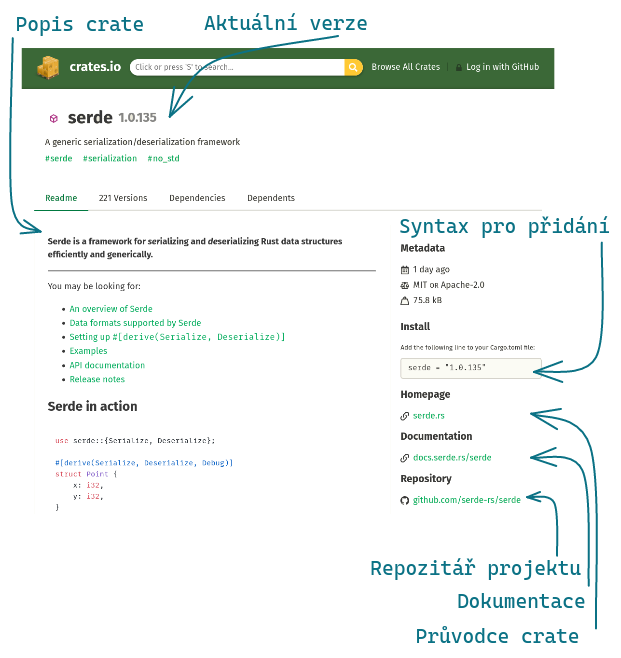
\includegraphics[width=0.95\linewidth]{cratesio}
					\caption{Ukázka a~popis crate serde na~\href{https://crates.io}{crates.io}}
					\label{fig:cratesio}
				\end{figure}
			\end{center}
			
			Avšak ještě je nutné vědět, jak s~danou crate zacházet. Na~stránce dané crate na~\href{https://crates.io}{crates.io} lze přečíst popis této crate, který většinou poskytuje minimalistickou ukázku kódu znázorňující zacházení s~ní. Avšak (pokud zde vůbec je) obsahuje minimální informace. Pro kompletní dokumentaci lze v~pravé části zpozorovat odrážku \texttt{Documentation}, obsahující odkaz na~dokumentaci dané crate, hostované na~\href{https://docs.rs/}{docs.rs}. Popřípadě, je-li crate kompletnější, může obsahovat jakéhosi průvodce, označeného v~pravé liště odrážkou \texttt{Homepage}.


		\subsubsection*{Dokumentace}
			Pro hlubší obeznámení s~jednotlivými crates je interakce s~přímou dokumentací nevyhnutelná. Není však nutné číst přímo zdrojový kód. Ekosystém poskytuje stránku \href{https://docs.rs}{docs.rs}, která autogeneruje nízkoúrovňovou dokumentaci přímo z~repozitářů. Lze zde najít i~\href{https://docs.rs/rustc-std-workspace-std/latest/std/index.html}{dokumentaci pro crate \rust{std}}. Například pro crate \rust{serde} vypadá takto
			
			\begin{center}
				\begin{figure}[H]
					\centering
					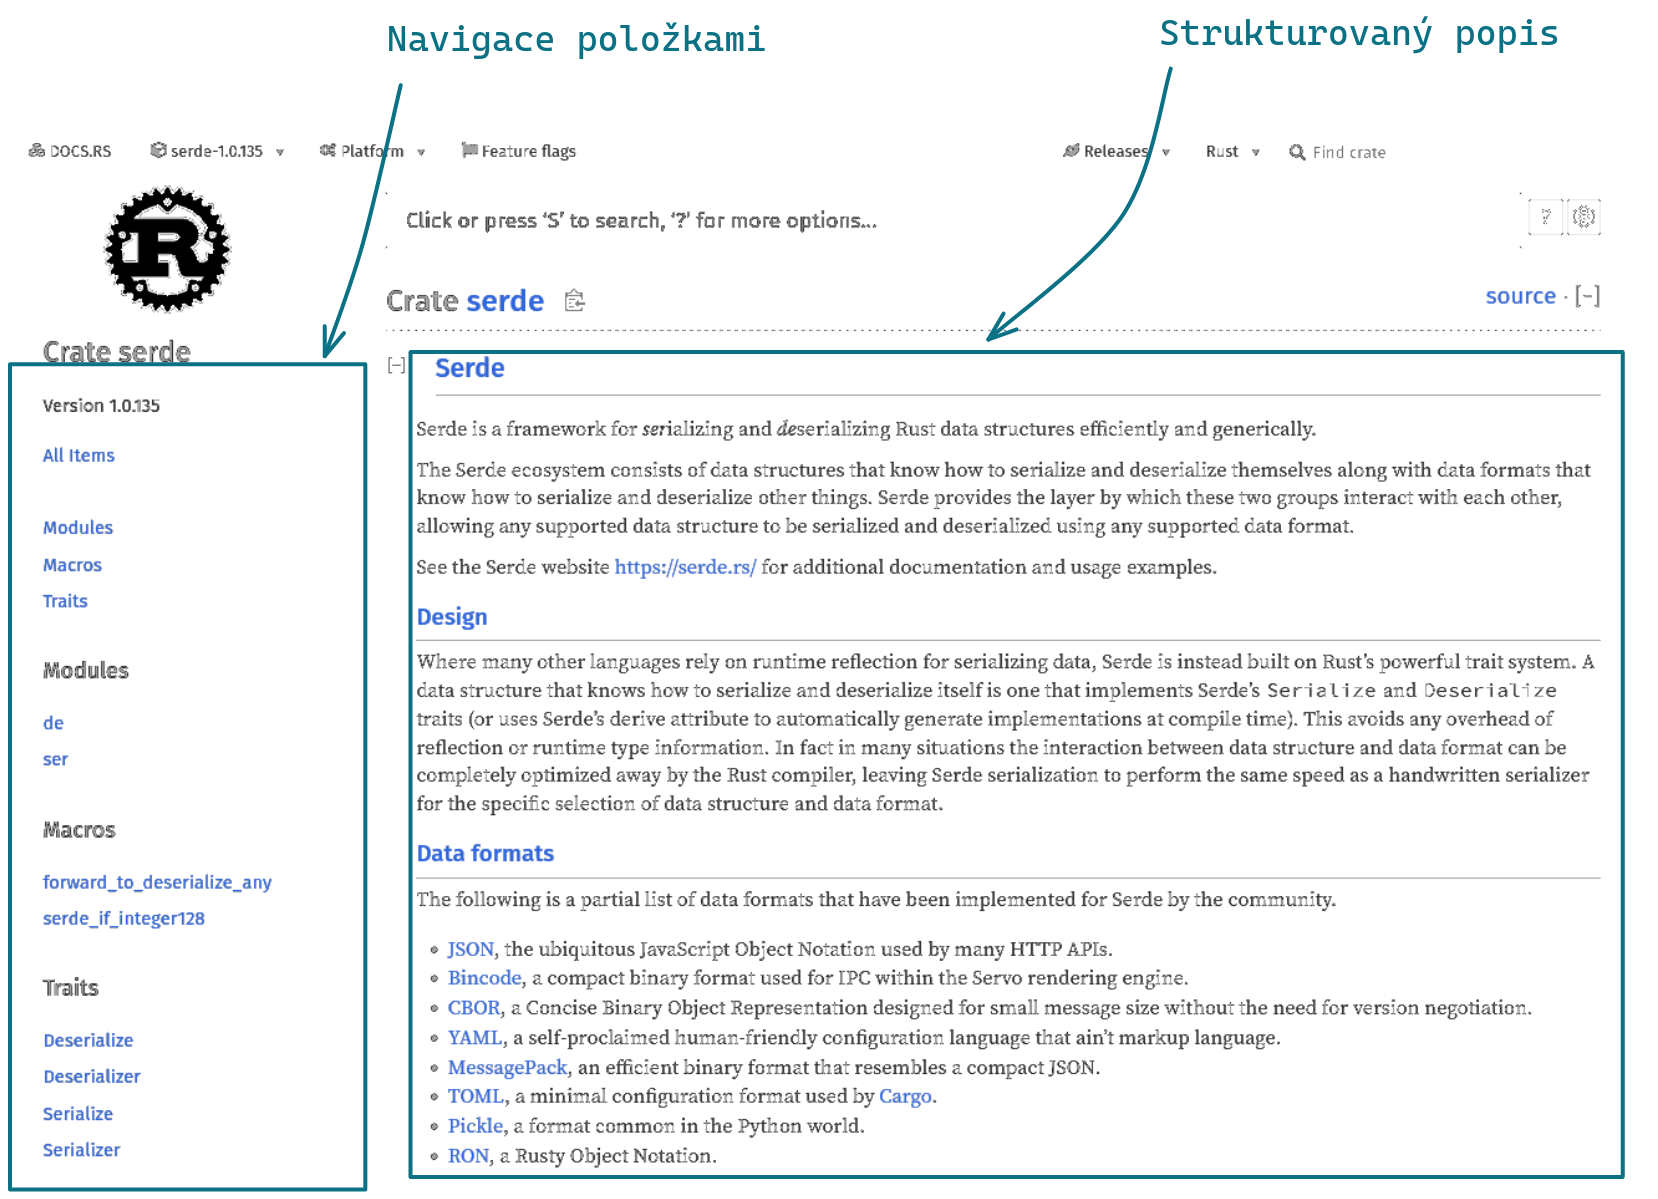
\includegraphics[width=\linewidth]{docsrs}
					\caption{Ukázka a~popis crate serde na~\href{https://docs.rs}{docs.rs}}
					\label{fig:docsrs}
				\end{figure}
			\end{center}


	\subsection{Zpracovávání chyb}
		Rust má poměrně sofistikovaný systém pro nakládání s~chybami. Nejdříve je však třeba si představit několik nových poznatků.

		struct nemusí být definován jen poli, ale může představovat jen jako pouhý alias nějakého tuplu. 
		\begin{minted}{rust}
struct Bod(f32, f32);

fn main {
	let bod = Bod(1., 0.7);
	println!("[{}, {}]", bod.0, bod.1);
}
		\end{minted}
		
		Nadále enumerační pole mohou držet také arbitrérní tuply
		\begin{minted}{rust}
struct Bod(f32, f32);

enum Obrazec {
	Trojuhelnik(Bod, Bod, Bod),
	Kruh(Bod, f32)
}

fn main() {
	let kruh = Obrazec::Kruh(
		Bod(0., 0.),
		3.
	);
}
		\end{minted}
			
		Je tedy vidno, že pole vskutku mohou držet hodnoty jakéhokoliv typu - klidně i~struct.

		S~tímto již lze přejít k~zpracovávání chyb. Prvním a~nejjednodušším způsobem zpracování a~identifikace chyb je enum \rust{Option}, který je ve zdrojovém kódu definován následovně
		\begin{minted}{rust}
pub enum Option<T> {
	None,
	Some(T),
}
		\end{minted}
		\cite{option_enum}

		Tento enum funguje pro vyjádření stavu nějaké hodnoty dané propměnné - buďto neexistuje, nebo existuje a~má nějakou hodnotu.
		\begin{minted}{rust}
struct MujStruct {
	hodn: Option<String>,
}

impl MujStruct {
	fn new() -> MujStruct { 
		MujStruct { hodn: None }
	} 

	fn udelat(&self) {
		if let Some(hodnota) = &self.hodn {
			println!("hodn je {}", hodnota);
		} else {
			println!("Hodnota není nastavena!");
		}
	}
}

fn main() {
	let mut a = MujStruct::new();
	a.hodn = Some("abvgd".to_string());
	a.udelat(); // hodn je abvgd

	let b = MujStruct::new();
	b.udelat(); // Hodnota není nastavena!
}
		\end{minted}

		Lze tedy vidět, že Option je použit jako chránič dané proměnné nebo atributu - je jím chráněna před tím, aby byla použita způsobem, který nemůže (nebo nemá smysl) vykonat.
		
		Pro pokročilejší (a závažnější) nečekaná chování a~chyby lze použít robustnější enum \rust{Result}.
		\begin{minted}{rust}
enum Result<T, E> {
	Ok(T),
	Err(E),
}
		\end{minted}
		
		Tento enum je generický a~nabývá buďto pole \rust{Ok(T)} obsahující danou hodnotu, pokud vyhodnocení operace bylo úspěšné, nebo pole \rust{Err(e)}, které nabyje pokud při vyhodnocování nastala nečekaná chyba (informaci o které obsahuje). Praktický příklad by mohl vypadat následovně.
		\begin{minted}{rust}
fn parse_na_int(s: &str) -> i32 {
	match s.parse() {
	// metoda `parse` se pokusí převést řetězec na číslo
	// pokud číslem hodnota je, vrátí `Result::Ok` s~danou hodnotou
	// pokud číslem hodnota není, vrátí `Result::Err` s~zprávou chyby
		Ok(n) => n,
		Err(e) => {
			println!("Vstup není číslo; nastavuji 0.\nChyba: {}", e);
			
			0
		}
	}
}

fn main() {
	let _ = parse_na_int("7");
	// proběhne v~pořádku

	let _ = parse_na_int("jovan");
	// Chyba: invalid digit found in string
}

// program vypíše:
// Vstup není číslo; nastavuji hodnotu na~0.
// Chyba: invalid digit found in string
		\end{minted}
		
		Pokud je v~daném kontextu nadevše jisté, že daná hodnota bude validní, poté lze použít metodu \rust{unwrap}.
		\begin{minted}{rust}
let _: i32 = "8".parse().unwrap();
// nastaví hodnotu proměnné `a` na 8 (i32)

let _: i32 = "abcd".parse().unwrap();
// způsobí runtime paniku se zprávou
// thread 'main' panicked at 'called `Result::unwrap()` on an `Err` value: ParseIntError { kind: InvalidDigit }'
		\end{minted}
		
		Pokud je deklarována vlastní funkce, která vrací \rust{Result}, postup může vypadat následovně.
		\begin{minted}{rust}
fn ctverec_ze_str(s: &str) -> Result<i32, std::num::ParseIntError> {
	match s.parse::<i32>() {
		Ok(n) => Ok(n.pow(2)),
		Err(e) => Err(e)
	}
}

fn main() {
	let a = ctverec_ze_str("42");

	if let Ok(cislo) = a~{
		println!("číslo je {}", cislo);
	} else {
		println!("není číslo");
	}
}
		\end{minted}
		
		Je tedy vidno, že výstup funkce je obalen enumem Result. Ten je specifikován typem i32, pokud je výstupem \rust{Ok} a~typem \rust{std::num::ParseIntError} pro případ, je-li výstupem \rust{Err}. Nadále je zde použito nového syntaxu co se týče metody parse. Je explicitně dán typ, do kterého se má parsovat (to proto, aby nebylo nutno nastavovat výsledek matche na~proměnnou požadovaného typu). Nadále je vrácena správná hodnota obalená enumem Result a~posléze je zpracována \rust{if let} výrazem. Tento koncept eskalování chyby se nazývá propagace chyb (error propagation).
		
		Tu lze syntakticky zjednodušit pomocí \rust{?} operátoru.
		\begin{minted}{rust}
fn ctverec_ze_str(s: &str) -> Result<i32, std::num::ParseIntError> {
	Ok(s.parse::<i32>()?.pow(2))
}
		\end{minted}

		V~tomto příkladu se funkce \rust{ctverec_ze_str} pokusí vrátit Ok, avšak když ve vyhodnocování výrazu dojde na~\rust{?}, je-li hodnota výrazu na~který je aplikován \rust{Ok(...)}, vrátí obsaženou hodnotu, ale je-li aplikován na~\rust{Err(...)} automaticky vystoupí z~funkce, ve které je použit, a~vrátí danou chybu \rust{Err(...)}. Pokud k~chybě nedošlo je dále hodnota v~této funkci zpracovávána a~je funkce \rust{ctverec_ze_str} je vráceno \rust{Ok(...)}.
		
		\subsubsection*{Defininování vlastních chyb}
			Zde je prerekvizitou možnost tvorby vlastních typů, například i~jakožto pouhý alias
			\begin{minted}{rust}
type MujTyp = String;
let a: MujTyp = "jovan".to_string();
			\end{minted}
		
			Toto nemá příliš smysl, ale nejčastějším využitím je pro Result, který lze implicitně nahradit vlastním „aliasem“.
			\begin{minted}{rust}
type Result<T> = std::result::Result<T, std::num::ParseIntError>;
			\end{minted}
			
			Takto je fixně dána hodnota Err-ového pole enumu Result a~následně se syntax výstupu funkce zjednodušuje na \rust{Result<i32>}.

			Kde je toto však nejvíce užitečné je při reprezentaci několika chyb najednou. Co se totiž stane, může-li v~jedné sekci kódu nastat více chyb (errorů)? Pro vyřešení tohoto problému lze vytvořit Result, který může nabýt kteréhokoliv z~enumem daných errorů.
			\begin{minted}{rust}
use std::error;
use std::error::Error as _;
use std::num::ParseIntError;
use std::fmt;

#[derive(Debug)]
enum VektorError {
	PrazdnyVektor,
	Parse(ParseIntError),
}

type Result<T> = std::result::Result<T, VektorError>;
			\end{minted}
			
			Nejprve je definován enum obsahující dané errory a~posléze je Err-ová složka vlastního Resultu nastavená na~tento enum. Enum je označený \rust{#[derive(Debug)]} pro automatické implementování traitu Debug (aby mohl být formátován pomocí \rust{:?}, více o tomto bude řečeno v~sekci o atributech).
			
			Následně je potřeba implementovat pro enum \rust{VektorError} další traits. Kromě Debug potřebují errory ještě mít implementovány traits Display a~\rust{std::error::Error}.
			\begin{minted}{rust}
impl fmt::Display for VektorError {
	fn fmt(&self, f: &mut fmt::Formatter) -> fmt::Result {
		match *self {
			VektorError::PrazdnyVektor =>
				write!(f, "vektor nesmí být prázdný"),
			VektorError::Parse(..) =>
				write!(f, "element není validní i32 číslo"),
		}
	}
}

impl error::Error for VektorError {
	fn source(&self) -> Option<&(dyn error::Error + 'static)> {
		match *self {
			VektorError::PrazdnyVektor => None,
			VektorError::Parse(ref e) => Some(e),
		}
	}
}
			\end{minted}

			Je tedy vidno, že implementace těchto traits zkrátka porovná o jaký typ chyby se jedná a~dle ní vykoná chtěný úkon. U~funkce \rust{source} v~implementaci  samotné \rust{std::error::Error} trait se nachází syntax, který je přiblížen v~sekci o chytrých ukazatelých.
			
			Jelikož jeden z~možných errorů je závislý na~již existujícím vestavěném erroru, je nutno implementovat převod tohoto erroru na vlastní.
			\begin{minted}{rust}
impl From<ParseIntError> for VektorError {
	fn from(err: ParseIntError) -> VektorError {
		VektorError::Parse(err)
	}
}
			\end{minted}
			
			Tím je hotovo. Následně by využití tohoto erroru mohlo vypadat nějak následovně
			\begin{minted}{rust}
fn vektor_do_cisel(v: Vec<&str>) -> Result<Vec<i32>> {
	if v.is_empty() {
		return Err(VektorError::PrazdnyVektor);
	}

	let mut vystup: Vec<i32> = Vec::new();

	for s~in v~{
		vystup.push(s.parse::<i32>()?);
	}

	Ok(vystup)
}

fn vypsat(r: Result<Vec<i32>>) {
	match r {
		Ok(v) => println!("Vektor má následující hodnoty {:?}", v),
		Err(e) => {
			println!("Při zpracování nastala následující chyba: {}", e);

			if let Some(zdroj) = e.source() {
				println!("Způsobeno: {}", zdroj);
			}
		}
	}
}

fn main() {
	let a = vec!["42", "777", "1453"];
	let b = vec![];
	let c = vec!["etrgt", "93", "18"];

	vypsat(vektor_do_cisel(a));
	// Vektor má následující hodnoty [42, 777, 1453]
	vypsat(vektor_do_cisel(b));
	// Při zpracování nastala následující chyba: vektor nesmí být prázdný
	vypsat(vektor_do_cisel(c));
	// Při zpracování nastala následující chyba: element není validní i32 číslo
	// Způsobeno: invalid digit found in string
}
			\end{minted}
			\cite{vice_typu}

			Bylo by dobré si povšimnout, že pro prázdný vektor nebyl vypsán žádný původce, jelikož v~implementaci funkce \rust{source} nebyl pro tuto variantu erroru žádný původce specifikován.


\section{Bezpečnost}
	\hypertarget{vlast}{}

	\subsection{Model vlastnictví}
		Některé programovací jazyky jako Java, Haskell nebo Go mají garbage collector (odvoz odpadu). Ten uvolňuje pamět zabranou proměnnými právě, když vyjdou z~rámce, v~kterém jsou definovány. Jiné jazyky nic takového neposkytují a~paměť musí být spravována přímo programátorem. Toto jsou jazyky jako C. Rust se liší od těchto dvou skupin tím, že vnutí přesná pravidla a~postupy dané modelem vlastnictví, díky čemuž kompilér ví přesně, kdy proměnná vychází z~jejího rámce, nebo životnosti (tzv. lifetime) a~na~základě toho použije adekvátní instrukce LLVM nebo jazyka symbolických adres (tento systém se označuje jako OBRM - ownership based resource management).
		
		\begin{center}
			\begin{figure}[H]
				\centering
				\includegraphics[width=.9\linewidth]{sprava_pameti}
				\caption{Různé strategie správy paměti \cite{sprava_pameti}}
				\label{fig:ret_mod}
			\end{figure}
		\end{center}
		
		Pro zachování bezpečnosti ohledně proměnných má Rust velice sofistikovaný a~specifický model vlastnictví. Je tomu tak, jelikož jeho filozofií je napsat o něco více kódu, což se však záhy vyplatí redukcí runtime chyb.
			
		Zprvu, již bylo na~některých místech před proměnnou užito znaku \rust{&}. Toto znaménko značí půjčení - každá proměnná hodnota je totiž vlastněna její proměnnou. Onu hodnotu lze půjčit (\rust{&} - reference), nebo půjčit s~možností změny (\rust{&mut} - mutable reference), nebo jí zkrátka „vzít“ jinou proměnnou. To, zda-li probíhají všechny tyto operace správně (dle pravidel) kontroluje při kompilaci \texttt{borrow checker}. Příkladem může být následující
		\begin{minted}{rust}
fn pridrzet(_: Vec<&str>) {}

fn main() {
	let jovan = vec!["Jovan", "Navoj", "Vojan"];
	pridrzet(jovan);

	println!("{:?}", jovan);
}
			\end{minted}
				
			Při spuštění tohoto kódu kompilér vrátí (nezkompiluje) následující chybu
			\begin{minted}{bash}
error[E0382]: borrow of moved value: `jovan`
	--> src/main.rs:7:22
	|
4 |     let jovan = vec!["Jovan", "Navoj", "Vojan"];
	|         ----- move occurs because `jovan` has type `Vec<&str>`, which does not implement the `Copy` trait
5 |     pridrzet(jovan);    
	|              ----- value moved here
6 | 
7 |     println!("{:?}", jovan);
	|                      ^^^^^ value borrowed here after move

For more information about this error, try `rustc --explain E0382`.
error: could not compile `muj_projekt` due to previous error
			\end{minted}
				
			Z chybového hlášení lze jasně přečíst následující: funkce \rust{pridrzet()} vezme hodnotu proměnné \texttt{jovan} (v argumentu při volání funkce není žádné \rust{&}), a~tedy je hodnota přesunuta. Z~tohoto důvodu není proměnnou \texttt{jovan} možné posléze použít. Řešení je jednoduché, změnit hlavičku funkce na~\rust{fn pridrzet(_: &Vec<&str>)} a~posléze při volání funkce použít referenci hodnoty proměnné \texttt{jovan} následovně \rust{pridrzet(&jovan)}.
				
			Rust má obecně velice přívětivý kompilér, který dává přesné chyby a~rady, pokud dojde k~chybě (respektive dává i~nápovědy, dojde-li k~nějaké kompilovatelné nestrovnalosti v~kódu).
			
			S~referencemi však může někdy dojít k~problémům, je-li referováno na~hodnotu, která již neexistuje (byla uvolněná z~paměti)
			\begin{minted}{rust}
fn visici_ref() -> &String {
	let s = String::from("Jovan");

	&s
}

fn main() {
	let reference_na_nic = visici_ref();
}
			\end{minted}
			\cite{dangle}
				
			Tento příklad se nezkompiluje. Při zahájení funkce je vytvořena proměnná typu \rust{String}. Posléze se tato funkce snaží vrátit referenci na~hodnotu této proměnné, avšak při posledním využití proměnné je uvolněna z~paměti, a~tedy odkazovat na~ní nemá smysl (adresa v~paměti bude přepsána něčím jiným).
	
			Borrow checker má následující pravidla
			\begin{itemize}
				\item v~jakýkoliv daný moment smí mít proměnná buďto 1 mutable referenci, nebo libovolný počet immutable (neměnitelných) referencí
				\item reference musí vždy být validní (tj. nesmí odkazovat na~neexistující proměnné)
			\end{itemize}
	
			Mohlo by se zdát podivné, vzhledem k~dřívějším úryvkům, proč nedojde k~zinvalidnění proměnné makrem \rust{println!}. Toto je dáno samotnou podstatou maker - toto makro slouží jako pouhá abstrakce pro zjednodušení syntaxe. Více o nich bude řečeno později.
			
		\subsection{Stack a~heap}
			Se znalostí modelu vlastností a~principu půjčování, lze již definovat rozdíl mezi \rust{String} a~\rust{str} (string slice) a~mezi \rust{Vec} a~\rust{&[]} (vector slice). Nejprve však stack a~heap.
				
			Zásobník (stack) je typ ukládání dat do paměti, kdy je daná hodnota do zásobníku nabita (push) a~posléze na~něj může být nabita další hodnota, nebo může být hodnota ze stacku vytlačena (pop). Avšak vždy lze operovat pouze s~hodnotou naposledy přidanou (tzv. LIFO model - Last In First Out).
			\begin{center}
				\begin{figure}[H]
					\centering
					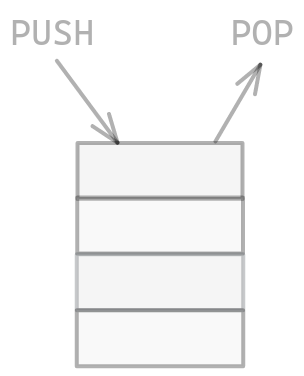
\includegraphics[width=4cm]{stack}
					\caption{Vizualizace správy paměti stack}
					\label{fig:my_label_2}
				\end{figure}
			\end{center}
				
			Druhým způsobem ukládání dat je heap (halda). Ta je naopak od stacku používána pro dynamicky se měnící hodnoty. Je to jakýsi region paměti, ke kterému může být postupně alokována další paměť.
				
			Obecně se tyto dvě struktury liší rychlostí - stack je znatelně rychlejší než heap, avšak nelze na~něj alokovat hodnoty neznámé velikosti (ty, které nejsou známé při kompilaci).
				
			Všechny základní numerické typy v~Rustu jsou uchovávány na~stacku. Avšak s~řetězci to není tak jednoznačné - kdykoliv je vytvořen řetězec, na~heap je přidán obsah a~zároveň je na~stack přidán pointer (reference) na~místo (počínající bod řetězce) v~heap a~délka řetězce (len)
				
			\begin{center}
				\begin{figure}[H]
					\centering
					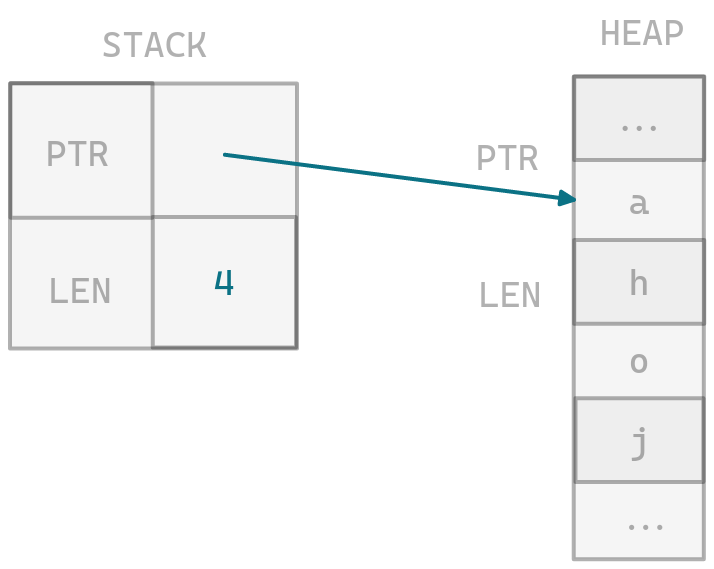
\includegraphics[width=6.5cm]{string_heap}
					\caption{Vizualizace vytvořeného řetězce znaků}
					\label{fig:my_label_3}
				\end{figure}
			\end{center}
				
			Část tohoto diagramu zobrazující stack je právě \rust{&str}. Toto je přesně typ, který je vracen inicializací jako \rust{let s = "ahoj"}. U~tohoto partikulárního příkladu je \rust{"ahoj"} pevně zakódovaný do binárního souboru vyprodukovaného po kompilaci a~při spuštění je načten do operační paměti. 
				
			Nadále
			\begin{minted}{rust}
let s = " jovan ";
let r = s.trim();
// `trim` je metoda pro odstranění mezer na konci a~začátku řetězce
			\end{minted}
				
			V~tomto příkladu je správa paměti velice efektivní, jelikož \texttt{r} vrátí \rust{&str}, jehož \texttt{ptr} ukazuje na~adresu písmene \texttt{j} a~jeho \texttt{len} je 5. Tím se obejde nutnost alokace nového prostoru v~paměti.
			\begin{minted}{rust}
let s = " jovan ";
let r = s.to_uppercase();
			\end{minted}
				
			Zde nemůže \rust{r} referovat na~původní řetězec ani jeho část, proto je naalokován pro tento typ nový prostor v~paměti a~je vrácen typ \rust{String}. \rust{String} je narozdíl od \rust{&str} dynamický a~lze ho měnit. To proto že je definován jako vektor 8-bitových čísel
			\begin{minted}{rust}
pub struct String {
	vec: Vec<u8>,
} 
			\end{minted}

			Obsah vektoru je vždy naalokován na~heap a~\rust{&[]} (vector slice) je pro něj tím, co je pro \texttt{String} \rust{&str} - lze ho použít pro nahlížení do svého dynamicky alokovaného protějšku.
			\begin{minted} {rust} 
let s = String::from("Jovan");
let ss = &s[2..4];
// &str odkazující na~znaky indexu 2 až 3 proměnné `s`, tedy "va"

let v = vec![5, 8, 2, 64, 10];
let vs = &v[..3];
// `&[]` odkazující na všechny indexy vektoru `v`
// mající index menší než 3, tedy [5, 8, 2]
			\end{minted}

			Samozřejmě tyto reference nelze měnit, jelikož dané hodnoty nevlastní, pouze na~ně ukazují.


		\subsection{Dereferenční operátor}
			Občas může nastat situace, kdy je žádáno získat hodnotu proměnné přímo, ač může být schována za referencí. K~tomu lze využít dereferenční ho operátoru \rust{*}
			\begin{minted}{rust} 
let jovan = 7;
let navoj = &jovan;

assert_eq!(jovan, *navoj);
			\end{minted}
		
		\subsection{Lifetime}
			Lifetime (životnost) je vyjádřením doby, kterou daná proměnná žije. Buď demonstrací tento příklad s~visící referencí
			\begin{minted}{rust}
fn main() {
	let t;

	{
		let u = 42;
		t = &u;
	}
	// pokud nejsou složené závorky {} nijak označené,
	// představují vlastní scope (rámec)

	// nic, co je vně těchto závorek, nemá přístup
	// k~ničemu inicializovanému v~tomto scope

	println!("{}", t);
}
			\end{minted}
			
			Tento příklad se nezkompiluje, jelikož by \rust{t} byla visící reference. Lifetimes proměnných \rust{t}, \rust{u} by vypadaly takto
			\begin{minted}{rust}
fn main() {
	let t;              // ---------+ 'a
						//          |
	{                   //          |
		let u = 42;     // -+ 'b    |
		t = &u;         //  |       |
	}                   // -+       |
						//          |
	println!("{}", t);  //          |
}                       // ---------+
			\end{minted}
			
			Lifetime \rust{t} je zde anotován jako \rust{'a} a~lifetime \rust{u} je anotován jako \rust{'b}. Diagram značí kde dané lifetimes začínají a~kde končí (tj. kde jsou proměnné zinvalidněny). Pomocí tohoto lze dovysvětlit visící referenci podrobněji - díky \rust{t = &u;} odkazuje \rust{t} na~\rust{u}, avšak \rust{u} nežije dostatečně dlouho na~to, aby mohla být využita její reference v~\rust{println!("{}", t);}.
			
			Konsekvencí lifetimes proměnných je nutnost jejich specifikace v~některých případech. Buď uvažován příklad
			\begin{minted}{rust}
fn nejvetsi(cislo1: &i32, cislo2: &i32) -> &i32 {
	if (cislo1 > cislo2) {
		cislo1
	} else {
		cislo2
	}
}

fn main() {
	let t = 7;
	let u = 42;
	
	println!("{}", nejvetsi(&t, &u));
}
			\end{minted}
			
			Anotace lifetimes je naprosto arbitrérní (musí však začínat s~\rust{'}), avšak dle konvence se značí malými počátečními písmeny latinské abecedy.
			
			Toto se nezkompiluje, a~to z~následujícího důvodu: Výstupem funkce \rust{nejvetsi()} je odkaz na~jednu z~proměnných, které jsou referencovány v~jejích parametrech. Avšak z~pohledu borrow checkeru, který kontroluje lifetimes, není jasné, jaké mají tyto vstupní parametry lifetimes. Co kdyby vracel odkaz proměnnou, která však nebude mít v~kontextu, ve kterém bude funkce použita, dostatečnou životnost? 
			
			Toto lze obejít anotací lifetimes v~hlavičce funkce \rust{nejvetsi()}.
			\begin{minted}{rust}
fn nejvetsi<'a>(cislo1: &'a i32, cislo2: &'a i32) -> &'a i32
			\end{minted}
			
			Tato syntaxe říká, že lifetime výstupní hodnoty bude stejný jako nejmenší lifetime proměnných, na~něž je odkazováno pomocí \rust{cislo1, cislo2}.
			
			Toto není samozřejmě jediný postup anotace. Ten se upraví dle způsobu, jakým má být funkce použita. Například pokud by bylo žádoucí svázat lifetime výstupu funkce s~lifetime jedného z~parametrů, šlo by to následovně.
			\begin{minted}{rust}
fn jovan<'a, 'b>(i: &'a mut str, j: &'b i32) -> &'b i32
			\end{minted}
			
			Lifetime anotace dovoluje také tvorbu structů, které nevlastní hodnoty svých polí
			\begin{minted}{rust}
struct Jovan {
	navoj: &str,
}

fn main() {
	let s = "abc";
	
	let i = Jovan {
		navoj: s
	};
	
	println!("{}", i.navoj);
}
			\end{minted}
			
			Toto by se nezkompilovalo, avšak po následné modifikaci ano.
			\begin{minted}{rust}
struct Jovan<'a> {
	navoj: &'a str,
}
			\end{minted}
			
			\subsubsection*{statický lifetime}
				Kdykoliv byla doposud použito řetězce takto \rust{let a= "b";}, tato proměnná neměla typ \rust{&str}, ale \rust{&'static str}. \rust{static} je speciální lifetime, který identifikuje, že daná hodnota je validní po celou dobu spuštění programu (což v~tomto případě je, jelikož, jak již bylo zmíněno, tyto hodnoty jsou pevně zakódované v~binárním souboru vyprodukovaným Rustem).


			\subsection{Doplňky ohledně modelu vlastnictví}
				Vstupní parametry anonymní funkce mohou být také označeny slovem \rust{move}. Poté closure všem proměnným, které jsou v~ní použity, vezme vlastnictví. 
				\begin{minted}{rust}
fn main() {
	let jovan = "Jovan".to_string();
	let a = move || println!("{}", jovan);

	println!("{}", jovan);
}
				\end{minted}

				Poslední řádek způsobí chybu a~příklad se nezkompiluje, jelikož při použití v~closure označeném jako \rust{move} bylo vlastnictví přesunuto.

\section{Pokročilé koncepty}
	\subsection{Multithreading}
		Rust je prominentní ve využití více vláken. S~vláknem (thread) lze zacházet pomocí \rust{std::thread}, minimální příklad by mohl vypadat následovně.
		\begin{minted}{rust}
fn main() {
	std::thread::spawn(|| {
		println!("jovan");
	});
}
		\end{minted}
		
		Je tedy vidno, že lze jednoduše využít funkce \rust{spawn}, která přijímá anonymní funkci, jejíž tělo se spustí v~daném vlákně. Je-li však vlákno takto spustěno, s~největší pravděpodobností program nic nevypíše. To je tím, že funkce \rust{main} může dokončit dříve než dané vlákno a~program skončí dříve, než se stihne daný thread ukončit. Toto lze obejít nastavením threadu na~nějakou proměnnou.
		\begin{minted}{rust}
fn main() {
	let t = std::thread::spawn(|| {
		println!("jovan");
	});
	
	t.join();
	// metoda `join` zaručí počkání na dokončení daného threadu
}
		\end{minted}
		
		Metoda \rust{join} dokonce vrátí Result, který je Err, jestli threadu nastala chyba a~Ok, nenastala-li. Takto lze získat hodnotu threadem vracenou.
		\begin{minted}{rust}
let t = std::thread::spawn(|| -> i32 { 42 });
println!("{}", t.join().unwrap()); // 42
		\end{minted}
		
		Nadále je potřeba zmínit typy anonymních funkcí. Ty se rozlišují dle traits, které představují.
		\begin{itemize}
			\item \rust{Fn} - všechny proměnné ve funkci jsou referencemi
			\item \rust{FnMut} - všechny proměnné ve funkci jsou měnitelné (mutable) reference
			\item \rust{FnOnce} - všechny proměnné ve funkci jsou vlastněné
		\end{itemize}
		
		Z tohoto důvodu je anonymní funkce threadu nutno označit slovíčkem \rust{move}, je-li chtěno, aby tato funkce měla přístup k~vnějším proměnným. \rust{move} vynutí, aby byla funkce interpretována jako FnOnce
		\begin{minted}{rust}
let i = 42;

let t = std::thread::spawn(move || {
	println!("{}", i);
});
		\end{minted}
		
		\subsubsection*{Kanály}
			Kanály (channels) jsou velice užitečným způsobem pro zrealizování situce při využití multithreadingu, kdy více vláken posílá nějakou informaci na~stejné místo. Tuto funkcionalitu umožňuje modul std::sync::mpsc (multiple producer, single consumer). Minimální příklad vypadá následovně.
			\begin{minted}{rust}
use std::sync::mpsc;

fn main() {
	let (sender, receiver) = mpsc::channel();
	
	sender.send(7).unwrap();
	sender.send(42).unwrap();

	println!("{:?}", receiver.recv().unwrap()); // 7
	println!("{:?}", receiver.recv().unwrap()); // 42
}
			\end{minted}
			
			Nejdříve jsou tedy vytvořeny dvě proměnné - jedna na~posílání (\rust{sender}) a~druhá na~přijímání (\rust{receiver}). Kdykoliv je kanálem vyslána hodnota \linebreak(\rust{sender.send(..)}), setrvává zde dokud není přijímačem přijata \linebreak(\rust{receiver.recv(..)}). Pokud by však v~této ukázce bylo přidáno ještě jednou \rust{receiver.recv(..)}, poté by došlo k~chybě, jelikož by přijímač čekal stále na~hodnotu, která nikdy nepřijde. Pro provenci takovéto situace lze použít místo metody \rust{recv} metodu \rust{try_recv}. Takto použita by vrátila \rust{Err(Empty)}.
			
			Avšak bylo řečeno, že funkcionalita existuje pro vlákna. Takový příklad by tedy vypadal následovně
			\begin{minted}{rust}
use std::sync::mpsc::channel;
use std::thread;
use std::time::Duration;

fn narocna_fce() -> i32 {
	thread::sleep(Duration::from_millis(2048));

	42
} 

fn main() {
	let (sender, receiver) = channel();
	let mut vysledek = 0;
	let mut vlakna = vec![];


	for _ in 0..10 {
		let sender_klon = sender.clone();

		let t = thread::spawn(move || {
			let cislo = narocna_fce();
			sender_klon.send(cislo).unwrap();
		});

		vlakna.push(t);
	}
	
	for vlakno in vlakna {
		vlakno.join().unwrap();
	}
	
	while let Ok(n) = receiver.try_recv() {
		vysledek += n;
	}

	println!("{}", vysledek); // 420
}
			\end{minted}
			\cite{kanaly}


	\subsection{Chytré ukazatele}
		Chytré ukazatele (smart pointers) jsou dalším způsobem pro správu paměti v~Rustu. Základním je již představená reference (\rust{&}). Tento ukazatel není ničím speciální, avšak chytré ukazatele jsou datastruktury, které mohou poskytovat funkcionality jako přidání metadat a~umožnění existence více vlastníků.
		
		Ve skutečnosti \rust{Vec} a~\rust{String} jsou chytrými ukazateli. Oba vlastní data, na~která ukazují, a~uchovávají další metadata jako např. kapacitu.
		
		\subsubsection*{\rust{Box}}
			\rust{Box} je chytrý ukazatel umožňující přidání hodnoty na~heap.
			\begin{minted}{rust}
let jovan = Box::new(5);
// na~heap je přidána hodnota 5 (i32)
// a~na~stack je uložen pointer odkazující na~lokaci v~heap

println!("{}", jovan);
			\end{minted}
			
			Hodnotu proměnné inicializované pomocí Boxu je možno používat, jelikož implementuje \rust{std::ops::Deref} trait.
			
			Praktičtější příklad by mohl být následovný (toto je jakousi implementací cons seznamu používaného v~funkcionálních jazycích jako Lisp)
			\begin{minted}{rust}
enum List {
	Cons(i32, List),
	Nil,
}

use List::{Cons, Nil};

fn main() {
	let list = Cons(1, Cons(2, Cons(3, Nil)));
}
			\end{minted}
			
			Tento příklad nezkompiluje. Je tomu tak, jelikož enum \rust{List} je rekurzivní - jeho pole \rust{Cons} obsahuje enum samotný. Rust však potřebuje znát velikost při kompilování, což u~rekurzivního objektu nelze. Lze toto však napravit pomocí Boxu
			\begin{minted}{rust}
enum List {
	Cons(i32, Box<List>),
	Nil,
}

use List::{Cons, Nil};

fn main() {
	let list = Cons(1, Box::new(Cons(2, Box::new(Cons(3, Box::new(Nil))))));
}
			\end{minted}
			\cite{box}
			
			Box lze také využít k~automatickému zpracování errorů
			\begin{minted}{rust}
use std::error;

type Result<T> = std::result::Result<T, Box<dyn error::Error>>;

fn udelat(s: &str) -> Result<(i32, char)> {
	Ok((
		s.parse::<i32>()?,
		s.chars().nth(3).ok_or("nemá 4. písmeno")?
		// chars převed &str na iterovatelné znaky

		// nth vrátí Option daného znaku na~indexu
		
		// ok_or převede Option<T, K> na Result<T, E>,
		// kde E je specifikovaný v~argumentu
	))
}

fn main() {
	let a = udelat("a");
	// Err(ParseIntError { kind: InvalidDigit })
	let b = udelat("123");
	// Err("nemá 4. písmeno")
}
			\end{minted}
			
			Tímto dynamickým řešením však dochází ke ztrátě výhody statického vyhodnocování chyb.\cite{box_err}
			
		\subsubsection*{Cell}
			Doposud byl dáno, že pokud není daný typ nebo objekt nastavený jako měnitelný pomocí \rust{mut}, poté ho nelze měnit. Tento systém je však limitující, ačkoliv je toto z~důvodu bezpečnosti paměti. Ale existují situace, kde by takové chování nemuselo být žádoucí. Tomuto se říká interior mutability (vnitřní měnitelnost). Užitečnost spočívá v~ situacích, kdy existuje například struct o větším počtu polí a~pouze 1 z~nich je žádáno být mutable, nebo například existuje-li metoda s~mutable referencí a~je žádáno navíc v~této metodě použít referenci, která není mutable.
			
			Jedním ze způsobů, jak tohoto dosáhnout, je pomocí \rust{Cell}. Příklad první ze zmíněných situací by mohl vypadat následovně
			\begin{minted}{rust}
use std::cell::Cell;

struct Vyrobek {
	nazev: String,
	vyrobce: String,
	cena: f32,
	rok_zahajeni: u16,
	// toto pole má smysl měnit
	je_v_prodeji: Cell<bool>,
}

fn main() {
	// není mutable
	let vyrobek = Vyrobek {
		nazev: "Vyrobek".to_string(),
		vyrobce: "Firma".to_string(),
		cena: 89.90,
		rok_zahajeni: 2022,
		je_v_prodeji: Cell::new(true),
	};

	// změní hodnotu
	vyrobek.je_v_prodeji.set(false);

	// metoda `get` vrátí kopii hodnoty
	assert_eq!(false, vyrobek.je_v_prodeji.get());
}
			\end{minted}
			\cite{cell}


		\subsubsection*{ReffCell}
			\rust{RefCell} (reference cell) je podobný jako Cell způsobem změny hodnoty, která není pod mutable vlastníkem, ale je kontrolován při runtimu, nikoliv při kompilaci. 
			\begin{minted}{rust}
use std::cell::RefCell;

struct Vyrobek {
	nazev: String,
	vyrobce: String,
	cena: f32,
	rok_zahajeni: u16,
	// toto pole má smysl měnit
	je_v_prodeji: RefCell<bool>,
}

fn main() {
	// není mutable
	let vyrobek = Vyrobek {
		nazev: "Vyrobek".to_string(),
		vyrobce: "Firma".to_string(),
		cena: 89.90,
		rok_zahajeni: 2022,
		je_v_prodeji: RefCell::new(true),
	};

	// změna pomocí replace
	vyrobek.je_v_prodeji.replace(false);

	// rychlé získání hodnoty
	println!("{}", *vyrobek.je_v_prodeji.borrow_mut());

	// změna pomocí replace_width, které přijímá closure
	vyrobek.je_v_prodeji.replace_with(|&mut b| !b);
	
	// rychlá změna
	*vyrobek.je_v_prodeji.borrow_mut() = true;
	
	let pujceni = vyrobek.je_v_prodeji.borrow_mut();
	let pujceni2 = vyrobek.je_v_prodeji.borrow_mut();
	// toto již není v~pořádku, pravidla o půjčování
	// jasně zakazují existenci dvou mutable referencí
}
			\end{minted}
			
			Ačkoliv se tato ukázka zkompiluje, poslední řádka způsobí následující runtime error.
			\begin{minted}{bash}
thread 'main' panicked at 'already borrowed: BorrowMutError', src/main.rs:34:41
			\end{minted}

		\subsubsection*{Mutex}
			Mutex funguje na~bázi vytvoření jedinečného přístupu k~hodnotě
			\begin{minted}{rust}
use std::sync::Mutex;

fn main() {
	let strazce = Mutex::new(42);
	
	// proměnná je zde uzamčena a~nelze s~ní manipulovat
	// jinak, než přes `zamek`
	let mut zamek = strazce.lock().unwrap();
	
	// změna hodnoty
	*zamek = 10;
	
	// čtení hodnoty
	assert_eq!(10, *zamek);
	
	// alternativně, aby nemusela být tvořena zbytečně
	// proměnná, lze pro rychlou změnu použít
	//  *strazce.lock().unwrap() = 10;
}
			\end{minted}
			
			To, že může existovat vždy jen jeden lock (zámek) lze demonstrovat následovně
			\begin{minted}{rust}
use std::sync::Mutex;

fn main() {
	let strazce = Mutex::new(42);

	let zamek1 = strazce.lock().unwrap();
	let zamek2 = strazce.lock().unwrap();
}
			\end{minted}
			
			Tento příklad se zkompiluje, avšak s~následujícím problémem: \rust{zamek2} nezpůsobí chybu, avšak čeká. Čeká do té doby, dokud \rust{zamek1} nezanikne, až poté se inicializuje. Pozor! Takovýto program, který nikdy první zámek neuvolní poběží donekonečna.
			
			Pokud je nutno vytvořit druhý lock, spíše je lepší využít \rust{try_lock} metody
			\begin{minted}{rust}
use std::sync::Mutex;

fn main() {
	let strazce = Mutex::new(42);

	let zamek1 = strazce.lock().unwrap();
	if let Ok(mut mutex) = strazce.try_lock() {
		*mutex = 30;
	};

	println!("{:?}", strazce);
	// Mutex { data: <locked>, poisoned: false, .. }

	// manuální uvolnění z~paměti
	std::mem::drop(zamek1);
	if let Ok(mut mutex) = strazce.try_lock() {
		*mutex = 30;
	};

	println!("{:?}", strazce);
	// Mutex { data: 30, poisoned: false, .. }
}
			\end{minted}
			
			\subsubsection*{RwLock}
				\rust{RwLock} (read-write lock) je podobný Mutexu s~tím rozdílem, že může přidělovat i~čtecí právo. Těchto čtecích zámků může být v~daný moment libovolný počet, avšak psací zámek může být pouze jeden.
				\begin{minted}{rust}
use std::sync::RwLock;

fn main() {
	let strazce = RwLock::new(42);

	let cteci_zamek1 = strazce.read().unwrap();
	let cteci_zamek2 = strazce.read().unwrap();

	assert_eq!(*cteci_zamek1, 42);
	assert_eq!(*cteci_zamek2, 42);

	std::mem::drop(cteci_zamek1);
	std::mem::drop(cteci_zamek2);


	let mut psaci_zamek1 = strazce.write().unwrap();
	*psaci_zamek1 += 7;
	println!("{}", psaci_zamek1); // 49
}
				\end{minted}
				
			\subsubsection*{Cow}
				\rust{Cow} (Copy on write) je chytrý ukazatel, který dokáže vrátit vlastněné, nebo půjčené hodnoty (čiže \rust{&str}, nebo \rust{String}, popřípadě \rust{&[]}, nebo \rust{Vec}).
				\begin{minted}{rust}
use std::borrow::Cow;

fn jovan(n: u8) -> Cow<'static, str> {
	match n {
		// metoda `into` pochází z~trait std::convert::Into
		// automaticky naformátuje do požadované výstupní
		// hodnoty
		42 => "42".into(),
		neco_jineho => format!("{}", neco_jineho).into(),
		// makro `format!` operuje jako println!,
		// ale vrátí String místo vypisování
	}
}

fn main() {
	for n in 41..45 {
		match jovan(n) {
			Cow::Borrowed(hodn) => println!("{}, výsl. je referován", n),
			Cow::Owned(hodn) => println!("{}, výsl. je vlastněn", n),
		}
	}
}
				\end{minted}
				\cite{cow}


			\subsubsection*{Rc}
				\rust{Rc} (reference counter) je chytrý ukazatel umožňující sdílení vlastnění hodnoty mezi více proměnnými
			
				\begin{minted}{rust}
use std::rc::Rc;

fn main() {
	let mut jovan = Rc::new(42);

	{
		let a = jovan.clone();
		let b = jovan.clone();
		// `clone` ve skutečnosti vytvoří nový
		// pointer na stejnou adresu v paměti

		println!("{}", Rc::strong_count(&jovan));
		// vypíše '3' - existují 3 ukazatele
	}

	// půjčení jako mutable
	let c = Rc::get_mut(&mut jovan).unwrap();

	*c += 1;
	assert_eq!(43, *jovan);
}
				\end{minted}
			
				V~pokročilejších případech se může vyplatit chytré ukazatel kombinovat. Takovým příkladem je použití RefCell uvnitř Rc. Takto je možné mít více vlastníků ve stejný moment, kteří mohou danou hodnotu měnit.
				\begin{minted}{rust}
use std::rc::Rc;
use std::cell::RefCell;

fn pripsat(s: Rc<RefCell<String>>) {
	let mut refer = s.borrow_mut();

	println!("{}", Rc::strong_count(&s));
	// vypíše '2' - existují 2 vlastníci

	refer.push('!');
}

fn main() {
	let j = Rc::new(RefCell::new("Jovan".to_string()));
	pripsat(Rc::clone(&j));

	println!("{:?}", j);
	// RefCell { value: "Jovan!" }
}
				\end{minted}


			\subsubsection*{Arc}
				\rust{Arc} (atomic reference counter) je velice užitečný chytrý ukazatel, který se hojně využívá, zejména při sdílení proměnných mezi různými vlákny. Operace využití stejné proměnné více vlákny totiž není standartně považována za bezpečnou, proto ji Rust nedovolí. Tato akce je možná pomocí kanálu, nebo pomocí Arc, který je predominantně použit v~kombinaci s~dalším chytrým ukazatelem, např. s~Mutexem.
				\begin{minted}{rust}
use std::sync::{Arc, Mutex};

fn main() {
	let s = Arc::new(Mutex::new(42));
	
	let z1 = Arc::clone(&s);
	let z2 = Arc::clone(&s);
	
	let t1 = std::thread::spawn(move || {
		for _ in 0..10 {
			*z1.lock().unwrap() += 1;
		}
	});

	let t2 = std::thread::spawn(move || {
		for _ in 0..10 {
			*z2.lock().unwrap() += 1;
		}
	});

	t1.join();
	t2.join();

	println!("{:?}", s);
	// Mutex { data: 62, poisoned: false, .. }
}
				\end{minted}
				\cite{mutex}
		
		
		%\subsubsection*{Definování vlastních chytrých ukazatelů}
			%Všechny chytré ukazatele jsou pouhými structy, které mají implementovaný traits \rust{Deref} a~\rust{Drop}.


	\subsection{Atributy}
		Atributy jsou malé úryvky kódu, které slouží pro metaprogramování jako automatického vytvoření vlastností specifikovaného structu, nebo například pro podmíněnou kompilaci. Následují syntax typu
		\begin{minted}{rust}
#[atribut = "hodnota"]
#[atribut(vlastnost = "hodnota")]
#[atribut(hodnota)]
		\end{minted}


		\subsubsection*{derive}
			Atribut \rust{derive} slouží k~automatické implementaci vlastností objektů. Buď uvažován následující příklad, kdy je za potřeby nahodilého vypsání objektu při vývoji
			\begin{minted}{rust}
struct Osoba {
	vek: u8,
	jmeno: String,
}

fn main() {
	let jovan = Osoba {
		vek: 7,
		jmeno: String::from("Jovan"),
	};
	
	println!("{:?}", jovan);
}
			\end{minted}
		
			Tento příklad nezkompiluje a~vrátí následující chybu
			\begin{minted}{bash}
error[E0277]: `Osoba` doesn't implement `Debug`
	--> src/main.rs:12:22
	|
12 |     println!("{:?}", jovan);
	|                      ^^^^^ `Osoba` cannot be formatted using `{:?}`
			\end{minted}
		
			Pro tento účel stačí přidat aplikovat na~\rust{struct Osoba} následující atribut
			\begin{minted}{rust}
#[derive(Debug)]
struct Osoba {
// ...
			\end{minted}
		
			Výstupem takto doplněného kódu by bylo
			\begin{minted}{bash}
Osoba { vek: 7, jmeno: "Jovan" }
		\end{minted}
		
			Pokud by však výstup měl být plnohodnotnou součástí finálního programu, bylo by zapotřebí pro daný objekt implementovat trait \rust{Display}. Ta slouží pro popis způsobu, jakým má být daný objekt vypsán.
			\begin{minted}{rust}
use std::fmt;

struct Osoba {
	vek: u8,
	jmeno: String,
}

impl fmt::Display for Osoba {
	fn fmt(&self, f: &mut fmt::Formatter) -> fmt::Result {
		write!(f, "Jmenuji se {} a~je mi {} let", self.jmeno, self.vek)
	}
}

fn main() {
	let jovan = Osoba {
		vek: 7,
		jmeno: String::from("Jovan"),
	};
	
	println!("{}", jovan);
	// vypíše 'Jmenuji se Jovan a~je mi 7 let'
}
			\end{minted}
			
			Toto lze zjednodušit pomocí \texttt{derive(Display)} z~externí crate derive\_more.
			\begin{minted}{rust}
use derive_more::{Display};

#[derive(Display)]
#[display(fmt = "Jmenuji se {} a~je mi {} let", jmeno, vek)]
struct Osoba {
	vek: u8,
	jmeno: String,
}

// ...
			\end{minted}

			Další (nativní) funkcionalitou derive je \rust{Copy}. Ten slouží pro bitového zkopírování daného objektu. Typicky
			\begin{minted}{rust}
#[derive(Debug)]
struct Nic;

fn main() {
	let a = Nic;
	let b = a;  // hodnota `a` je přesunuta sem
	
	println!("{:?}", a);
	// chyba! nezkompiluje se (hodnota byla přesunuta jinam)
}
				\end{minted}
			
				Do derive však stačí přidat \rust{Copy}
				\begin{minted}{rust}
#[derive(Debug, Copy)]
				\end{minted}
			
				A následně na~řádku \rust{let b = a;} dojde ke zkopírování proměnné \rust{a} a~tím není nikam \texttt{a} přesunuta a~program se zkompiluje.

				Mezi další vlastnosti sdružené pod derive patří např. \rust{PartialEq}, \rust{Clone}, ad. Jednotlivé crates mohou přidávat k~dispozici další.


		\subsubsection*{Povolení nežádoucího kódu}
			Většina předchozích ukázek kódu by, pokud nebylo řečeno jinak, se zkompilovala, avšak kompilér by vrátil nějaká varování. To je proto, že ačkoliv může kompilér povolit nějaké chování, neznamená to, že by se toto chování mělo vyskytovat v~(finální verzi) programu. Buď příkladem
			\begin{minted}{rust}
fn main() {
	let s = "ahoj";
}
			\end{minted}
			
			Toto by se zkompilovalo, avšak bylo by vráceno varování
			\begin{minted}{bash}
warning: unused variable: `s`
	--> src/main.rs:2:9
	|
2 |     let s = "ahoj";
	|         ^ help: if this is intentional, prefix it with an underscore: `_s`
	|
	= note: `#[warn(unused_variables)]` on by default
			\end{minted}
			
			Je vidno, že kompilér dokonce i~radí, jak se zachovat dle konvencí - pokud je toto schválně, lze buďto připsat \rust{_} na~začátek jména proměnné, nebo, jak je viďet na~posledním řádku ukázky, lze změnit vlastnost \rust{unused_variables}. Tu lze změnit přidáním následujícího atributu do hlavičky daného souboru
			\begin{minted}{rust}
#[allow(unused_variables)]
			\end{minted}
			
			Toto zaručí, že všechny proměnné v~souboru definované, které nejsou použité, nepodnítí kompilér k~vrácení varování.
			
			Další podobné atributy jsou
			\begin{itemize}
				\item \rust{dead_code} - nevyužité vzory jako structy nebo funkce
				\item \rust{unused_mut} - žadná změna proměnné, která je definovaná s~\rust{mut}
				\item \rust{non_snake_case, non_camel_case_types} - nedodržení konvence názvů (viz \hyperlink{konvence_nazvu}{příloha})
			\end{itemize}

		\subsubsection*{Podmíněná kompilace}
			Pomocí atributů lze specifikovat, zda-li mát být daná sekce kódu (většinou funkce) zkompilována. Toto je zejména využito při vývoji cross-platform programu, ale je také vhodná, je-li daný projekt velký a~poskytuje spoustu funkcionalit a~při kompilování jsou žádoucí jen některé z~nich.
			\begin{minted}{rust}
#[cfg(target_arch = "windows")]
fn cesta_k_souboru() { /* ... */ }

#[cfg(target_arch = "linux")]
fn cesta_k_souboru() { /* ... */ }
			\end{minted}
			
			Při kompilaci do dané architektury (více o exportu funkcí v~sekci \hyperlink{cross-platform}{Cross-platform export aplikací}) je nastavena hodnota \rust{target_arch} atributu \rust{cfg}, načež je využitá správná definice funkce \rust{cesta_k_souboru}.
			
			Vlastní funkcionality lze využít následovně
			\begin{minted}{rust}
#[cfg(feature = "mojeFunkcionalita")]
fn jovan() { /* ... */ }

#[cfg(feature = "mojeDalsiFunkcionalita")]
struct Navoj { /* ... */ }
			\end{minted}
			
			Poté, mají-li části kódu označené touto feature být zkompilovány, musí se v~souboru \texttt{Cargo.toml} objevit pod nějakým označením
			\begin{minted}{toml}
[features]
extra = ["mojeFunkcionalita", "mojeDalsiFunkcionalita"]
			\end{minted}
			
			a následovně chceme-li tyto features, opravdu zkompilovat, nutno přidat vlajku \texttt{--features <nazev>}, takže například
			\begin{minted}{bash}
cargo build --release --features extra 
			\end{minted}
			
			Kdyby těchto kolekcí bylo více, které je žádané zkompilovat, lze je v~tomto výrazu oddělit čárkou. např.: \texttt{--features extra,experimentalni} 


	\subsection{Makra}
		Již byly několikrát zmíněna makra. Ta slouží k~metaprogramování a~generování kódu. V~Rustu existují dva typy maker - deklarativní a~procedurální. Procedurální přijme nějaký vstup a~porovnává ho se vzory, dle čehož vygenerují nějaký kód, kdežto deklarativní srovnají vstup se vzory, načež nahradí daný kód.


		\subsubsection*{Deklarativní makra}
			Příkladem bylo mohlo být
			\begin{minted}{rust}
#[macro_export]
macro_rules! c {
	() => {
		println!("Ahoj");
	};

	($arg1:ident) => {
		let $arg1 = 0;
	};
	
	($arg1:ty => $arg2:ident ! $arg3:expr) => {
		let $arg2: $arg1 = $arg3;
	}
}

fn main() {
	c!();
	// println!("ahoj");
	
	c![jovan];
	// let jovan = 0;
	
	c! {u32 => navoj ! 7};
	// let navoj = 7;
}
			\end{minted}

			Nejprve je užito atributu \rust{macro_export}. Ten dovolí makro použít ve funkci \rust{main} (a přidružených). Nebylo-li by tak učiněno, makro by bylo možné použít jen souřadně s~definicí makra. V~těle definice lze definovat libovolné množství vzorů označených \rust{()}. Při invokaci makra dochází k~porovnáváním se vzory a~první, který splňuje syntax, je aktivován. Pokud dojde k~invokaci makra výrazem, který nevyhovuje žádnému ze vzorů, dojde ke compile-time chybě. Parametry se označují \texttt{\$}, následuje jejich název (libovolný), který je pomocí \texttt{:} oddělen od jeho tzv. fragmentového specifikátoru. Tyto jsou pevně dány. Nejběžnější z~nich jsou
			\begin{itemize}
				\item \rust{ident} - identifikátor (název/označení), např. \rust{jovan}
				\item \rust{expr}  - výraz - výraz, např. \rust{1+1} nebo \rust{if (1>2) {true}}
				\item \rust{ty}    - typ, např. \rust{u32} nebo \rust{bool}
				\item \rust{pat}   - vzor, např. \rust{Some(i)} nebo \rust{_} (\hyperlink{_}{viz})
				\item \rust{meta}  - meta prvek, jako atributy
			\end{itemize}\cite{makra}
			
			Jednotlivé argumenty jsou ve vzoru odděleny tokeny, které jsou volitelné a~mohou být jakékoliv, dokud v~Rustu existují (\rust{?}, \rust{(}, \rust{as}, \rust{where}, \rust{=>}, \dots), za předpokladu, že jsou dodržena následující pravidla
			\begin{itemize}
				\item \rust{expr} a~\rust{stmt} mohou být následovány jen \texttt{=> , ;}
				\item \rust{ty} a~\rust{path} mohou být následovány jen \texttt{=> , = ; : > [ \{ as where}
				\item \rust{pat} může být následován jen \texttt{=> , = | if in}
			\end{itemize}
			
			V~poslední řadě si lze všimnout, že při volání makra mohou být použité ruzné závorky - \rust{()}, \rust{{}} nebo \rust{[]}.
			
			Tento příklad byl však poněkud minimální a~nepřidával makrům jejich skutečnou výhodu. Tou je možnost akceptování dynamických škálovatelních vstupů. Např.
			\begin{minted}{rust}
#[macro_export]
macro_rules! c {
	($($i:expr),*) => { 
		$(
			println!("{}", $i);
		)*
	};
}


fn main() {
	c!("jovan", "navoj", "javon");
	// println!("{}", "jovan");
	// println!("{}", "navoj");
	// println!("{}", "javon");
}
			\end{minted}
			
			\rust{($($i:expr),*)} znamená, že se v~parametru vyskytuje 0 a~více čárkou oddělených výrazů. Následně je v~expanzi vzoru užito \texttt{\$(\dots)*}. Podstata tohoto syntaxu spočívá v~tom, že výraz v~závorkách je opakován přesně tolikrát, kolikrát se proměnná, kterou obsahuje, vyskytuje v~parametrech. Místo kvantifikátoru \rust{*} by také mohlo být použito \rust{+}, to však slouží jen pro ty případy, kdy musí být aspoň jeden parametr (dle daného příkladu by fungovalo i~pouhé \rust{c!()}, avšak při použití kvantifikátoru \rust{+} by \rust{c!()} bylo chybou).
			
			Praktičtějším příkladem by bylo následující. Buď dáno
			\begin{minted}{rust}
trait MaxHodnota {
	fn max_hodn() -> Self;
}
			\end{minted}
			
			Bylo by však nepraktické explicitně implementovat tuto trait pro každý číselný typ (respektive každý, pro který je implementace žádána).
			\begin{minted}{rust}
impl MaxHodnota for i8 {
	fn max_hodn() -> i8 {
		i8::MAX
	}
}

impl MaxHodnota for i16 {
	// ...
}

// ...
			\end{minted}
			
			Pro zkrácení tohoto zbytečně dlouhého (a ne přílíš změnám susceptibilního) příkladu lze zjednodušit následovně
			\begin{minted}{rust}
trait MaxHodnota {
	fn max_hodn() -> Self;
}

macro_rules! max_impl {
	($($t:ty)*) => {
		$(impl $crate::MaxHodnota for $t {
			fn max_hodn() -> Self {
				<$t>::MAX
			}
		})*
	}
}

max_impl! {
	usize u8 u16 u32 u64 u128 isize i8 i16 i32 i64 i128 f32 f64
}

fn main() {
	println!("{}", i32::max_hodn()); // 2147483647
	println!("{}", u64::max_hodn()); // 18446744073709551615
}
			\end{minted}
			
			Zde přibývá několik další poznatků ohledně syntaxu maker. Pokud není oddělovač specifikován, jako v~\rust{($($t:ty)*)} před \rust{*}, je použit výchozí oddělovač - mezera. Dálé lze použít \texttt{\$crate::} pro odkaz na~položku nacházející se v~dané crate a~také je nutno typ ve výrazu obalit \rust{<>}. Mimochodem toto partikulární makro ušetří 61 řádků kódu a~navíc k~tomu je ním daná funkcionalita jednodušeji upravitelná.\cite{dekl_makra}

		\subsubsection*{Procedurální makra}
			Procedurální makra dokáží dělat spoustí věcí, které deklarativní nedokáží. Avšak nevýhodou je, že používají externích crates jako \rust{syn} pro tokenizace Rustového kódu, kvůli čemuž je daný projekt ihned objemnější, a~tedy náročnější na~kompilaci (nikoli však pro runtime).
			
			Rozlišují se tři základní typy
			\begin{itemize}
				\item funkcionální - jsou volány stejně jako makra deklarativní (\texttt{priklad!(..)})
				\item derivovací - jsou volány jako derive atributy (\texttt{\#[derive(priklad)]})
				\item atributivní - využívají vlastního atributu pro volání (\texttt{\#[priklad]})
			\end{itemize}
			
			Procedurální makra, narozdíl od deklarativních, tzv. nejsou hygienické. To znamená, že mezi jejich kódem a~kódem crates, do nichž jsou importovány, může dojít ke kolizi. Proto by názvy nimi generované měli být volené tak, aby k~těmto kolizím dojít nemohlo, \rust{__treba_takto}.
			
			Nadále procedurální makra musejí být vždy v~crate označené jako crate obsahující procedurální makra. Tedy lze postupovat následovně. V~adresáři projektu se vytvoří nová lib crate
			\begin{minted}{bash}
cargo new --lib moje_makro
			\end{minted}
			
			Poté bude struktura projektu vypadat následovně
			\begin{center}
				\begin{forest}
					for tree={
					font=\ttfamily,
					grow'=0,
					child anchor=west,
					parent anchor=south,
					anchor=west,
					calign=first,
					edge path={
						\noexpand\path [draw, \forestoption{edge}]
						(!u.south west) +(7.5pt,0) |- node[fill,inner sep=1.25pt] {} (.child anchor)\forestoption{edge label};
					},
					before typesetting nodes={
						if n=1
						{insert before={[,phantom]}}
						{}
					},
					fit=band,
					before computing xy={l=15pt},
					}
				[muj\_projekt
					[.git
					[\vdots]
					]
					[moje\_makro
					[src
						[lib.rs]
					]
					[Cargo.toml]
					]
					[src
					[main.rs]
					]
					[.gitignore]
					[Cargo.toml]
				]
				\end{forest}
			\end{center}
			
			Nejprve je nutno v~\texttt{Cargo.toml} (uvnitř složky \texttt{moje\_makro}) specifikovat, že se jedná o crate s~procedurálními makry. Pro používání procedurálních maker je užito externích crates jako proc-macro2 pro lepší podporu tvorby maker, crates pro parsování, převod na~syntaktický strom (syn) a~následnou zpětnou tokenizaci zdrojového kódu (quote).
			\begin{minted}{toml}
[lib]
proc-macro = true

[dependencies]
syn = { version = "1.0", features = ["extra-traits", "full"] }
quote = "1.0"
proc-macro2 = "1.0"
			\end{minted}
			
			(Některé z~těchto crates nebudou použity hned, ale až v~dalších příkladech procedurálních maker.) Poté stačí na~tuto crate odkázat v~\texttt{Cargo.toml} hlavní crate pro možnost využití kódu z~\texttt{moje\_macro}
			\begin{minted}{bash}
moje_makro = { path = "moje_makro" }
			\end{minted}

			Nejprve funkcionální makra: v~souboru \texttt{lib.rs} vytvoří dané makro (které pro nyní je pouze inspirativní)
				\begin{minted}{rust}
extern crate proc_macro;
use proc_macro::TokenStream;

#[proc_macro]
pub fn vytvorit_jovan(_item: TokenStream) -> TokenStream {
	"fn jovan() -> &'static str { \"navoj\" }".parse().unwrap()
}
			\end{minted}
				
			Následně ho lze naimportovat z~\texttt{main.rs} a~využít
			\begin{minted}{rust}
use test_procmac::make_answer;

vytvorit_jovan!();
//  fn jovan() -> &'static str {
//      "navoj"
//  }

fn main() {
	println!("{}", jovan());
	// vypíše 'navoj'
}
			\end{minted}
			\cite{fcialni_proc}
				
			Ačkoliv toto zatím není příliš praktické, je zde však vidět to, co činí procedurální makra odlišnými. Funkcí definované makro vezme jakožto vstup nějaký \rust{TokenStream} - tím je nějaký struct nebo třeba enum a~výstupem této funkce je další TokenStream. V~následující implementaci derive makra bude vstupem funkce TokebStean, jenž je ve své definici označen daným derive atributem, výstupní TokenStream bude následně přidán do modulu, v~němž se nachází daný vstupní TokenStream.
			\begin{center}
				\begin{figure}[H]
					\centering
					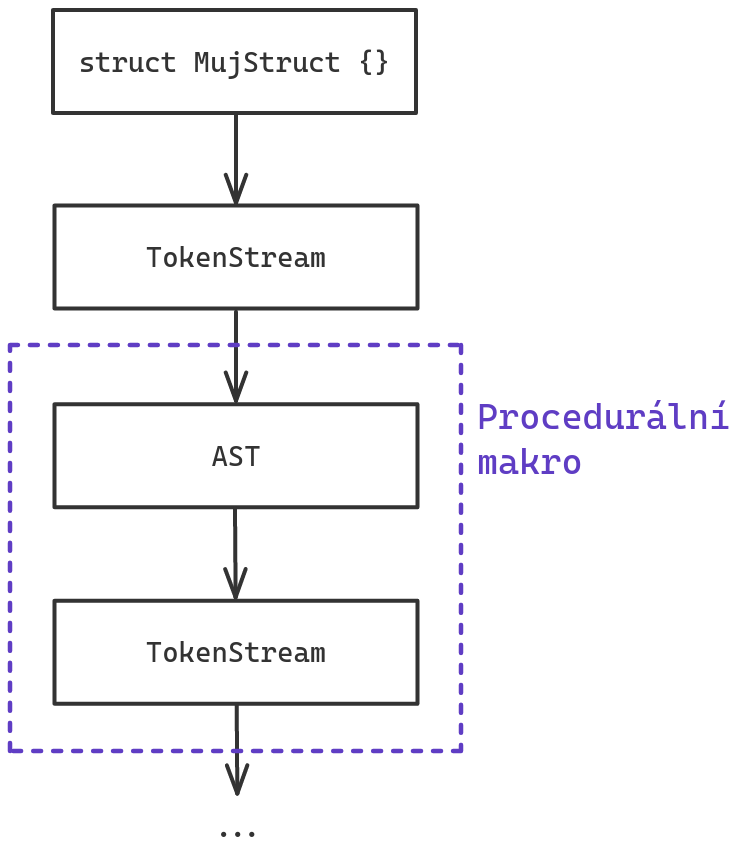
\includegraphics[width=7cm]{proc}
					\caption{Procedurální makra v~kontextu kompilačního procesu}
					\label{fig:proc}
				\end{figure}
			\end{center}
			
			Nadále makra derivativní: nejprve je nutno si vymezit cíle. Bude tvořeno makro, které dokáže převést řetězce libovolného structu na~jeden velký, je zamýšleno, aby použití vypadalo takto
			\begin{minted}{rust}
#[derive(Spojit)]
struct Kniha {
	nazev: String,
	autor: String,
	popis: String
}
			\end{minted}

			Navíc požadavkem je, aby se pole structu mohla jmenovat jakkoliv a~mohlo by jich být libovolně velké množství.

			Nuže v~\texttt{lib.rs} se začne takto
			\begin{minted}{rust}
extern crate proc_macro;
use proc_macro::{TokenStream};
use quote::quote;
use syn::{parse_macro_input, DeriveInput, FieldsNamed};

#[proc_macro_derive(Spojit)]
pub fn spojit(tokens: TokenStream) -> TokenStream {
	// převod na abstraktní syntaktický strom
	let ast = parse_macro_input!(tokens as DeriveInput);
	
	println!("{:#?}", ast);

	TokenStream::new()
}
			\end{minted}
			
			Tentokrát je funkce definující makro však označena jako \linebreak\texttt{\#[proc\_macro\_derive(..)]}. Nadále je velice důležité získat znalost opravdové struktury kódu - tak, jak na~ni nahlíží kompilér. Tím je asymptotický syntaktický strom, který je tímto kódem vypsán. Ačkoliv definice structu \rust{Kniha} ve zdrojovém kódu zabírá pouhých 5 řádků, expanze tohoto kódu, jak lze zjistit spuštěním předešlého kódu, je celých 183 řádků. To však při parsování AST dovoluje plnou kontrolu. \rust{TokenStream::new()} je pouze prozatímní. Začátek vypsaného AST vypadá takto.
			\begin{minted}{rust}
DeriveInput {
	attrs: [],
	vis: Inherited,
	ident: Ident {
		ident: "Kniha",
		span: #0 bytes(47..52),
	},
			\end{minted}
			
			Čiže je vidno, že se jedná o jakýsi struct, k~jehož polím lze přistupovat. Tento objekt je pomalu nutno parsovat k~dosáhnutí požadované funkcionality. Finální makro bude vypadat takto
			\begin{minted}{rust}
#[proc_macro_derive(Spojit)]
pub fn spojit(tokens: TokenStream) -> TokenStream {
	// převod na abstraktní syntaktický strom
	let DeriveInput { ident, data, .. } = parse_macro_input!(tokens);

	// parsování ast
	let vysl = match data {
		syn::Data::Struct(s) => match s.fields {
			syn::Fields::Named(FieldsNamed { named, .. }) => {
				let idents = named.iter().map(|i| &i.ident).map(|i| quote! {self.#i.clone()});
				// vrácení TokenStreamu makrem quote::quote
				// vnější proměnné jsou značeny pomocí #
				quote! {
					impl #ident {
						pub fn spoj(&self) -> String {
							// syntax pro rozvoj jako u~deklarativních maker
							[#(#idents),*].join("")
						}
					}
				}
			},
			_ => panic!("makro použito na invalidní datastrukturu")
		},
		_ => panic!("makro použito na invalidní datastrukturu")
	};

	vysl.into()
}
			\end{minted}
			
			A využití bude vypadat následovně
			\begin{minted}{rust}
use moje_makro::Spojit;

#[derive(Spojit)]
struct Kniha {
	nazev: String,
	autor: String,
	popis: String
}

fn main() {
	let kniha = Kniha {
		nazev: "孫子".into(),
		autor: "孫子兵法".into(),
		popis: "是中國古代的兵書".into(),
	};

	println!("{}", kniha.spoj());
	// 孫子孫子兵法是中國古代的兵書
}
			\end{minted}
			\cite{atrib_makro}
			
			Stejně tak by makro fungovalo na~jakýkoliv další struct, který má libovolný počet polí, která jsou všechna typu String. Kvůli spoustě parsování a~náročnějšímu syntaxu je velmi užitečné využití programu cargo-expand popsaného v~kapitole Troubleshooting.
			
			Atributivní makra jsou velice podobná těm derivativním, avšak jsou více flexibilní. Například ve frameworku rocket (sloužící pro vývoj webových aplikací) jsou použity následovně: 
			\begin{minted}{rust}
#[get("/hello/<name>/<age>")]
fn hello(name: &str, age: u8) -> String {
	format!("Hello, {} year old named {}!", age, name)
}
			\end{minted}
			\cite{rocket}
			
			Jde vidět, že při zadání atributu lze využít parametrů specifických pro danou situaci (v tomto případě pro udání cesty URI). Tato makra se také vytvářejí podobně. Avšak s~tím, že funkce makro definující je deklarována následovně.
			\begin{minted}{rust}
#[proc_macro_attribute]
fn moje_makro(meta: TokenStream, input: TokenStream) -> TokenStream {
	input
} 
			\end{minted}
			
			Zde \rust{input} je klasický TokenStream structu a~proměnná \rust{meta} obsahuje případné hodnoty udané v~argumentu atributu (také jakožto TokenStream). Tyto hodnoty se získají následovně: má-li být hodnota specifikována nějak takto \linebreak\texttt{\#[moje\_makro(cesta = "../assets/javor.png")]}, poté k~hodnotě \rust{cesta} v~tělu makra lze přistoupit takto
			\begin{minted}{rust}
let parametry_makra = syn::parse_macro_input!(meta as MacroParameters);
let sql_filename = macro_parameters.sql.as_str();
// dle předchozího příkladu by sql_filename nabyla
// hodnoty '"../assets/javor.png"'
			\end{minted}
			\cite{atrib_makro}
			
			U~atributivních i~deklarativních maker lze navíc využít pomocných atributů. Například pro to, aby nějaké pole bylo jinak procesováno než ta ostatní. Buď uvažována modifikace příkladu derivativních maker
			\begin{minted}{rust}
#[derive(Spojit)]
struct Kniha {
	nazev: String,
	autor: String,
	popis: String,
	#[nebrat]
	rok_vydani: u16
}
			\end{minted}
			
			
			Poté by se musela změnit definice makra \texttt{Spojit} následovně.
			\begin{minted}{rust}
#[proc_macro_derive(Spojit, attributes(nebrat))]
			\end{minted}
			
			Poté by tato informace byla možná vyparsovat ze vzniklého AST.\cite{atrib_makro}


\section{Troubleshooting}
	Co se týče psání kódu, je v~Rustu občas možné dostat se do rozpaků. Pro vyřešení tohoto lze použít několik metod.


	\subsection{Testování}
		Testování je důležitou metodou při vývoji programu. Zejména obtížné může být situace, kdy je psán kód (sekce kódu), jehož funkci by bylo obtížné prakticky důkladně ověřit. Proto je vhodné využít jednotkové testování (unit testing).
		
		Nejdříve je nutno seznámit se s~3 základními makry
		\begin{itemize}
			\item \rust{panic!}
				\begin{itemize}
					\item přijímá 1 argument - \rust{&str}
					\item způsobí konec programu se zprávou danou argumentem
				\end{itemize} 
			\item \rust{assert!}
				\begin{itemize}
					\item přijímá 1 argument - \rust{bool}
					\item pokud je argument \rust{false}, zpanikaří, jinak neudělá nic
				\end{itemize}
			\item \rust{assert_eq!}
				\begin{itemize}
					\item přijímá 2 argumenty - libovolné výrazy
					\item pokud sledá argumenty neidentickými, zpanikaří, jinak neudělá nic
				\end{itemize}
			\item \rust{assert_ne!}
				\begin{itemize}
					\item přijímá 2 argumenty - libovolné výrazy
					\item pokud sledá argumenty identickými, zpanikaří, jinak neudělá nic
				\end{itemize}
		\end{itemize}

		Pro testování je konvencí vytvořit v~souboru s~testovaným kódem speciální modul. Relativně praktický případ by mohl vypadat následovně
		\begin{minted}{rust}
struct Kruh {
	r: f32,   
}

struct Ctverec {
	a: f32
}

impl Ctverec {
	fn vejde_se_do_kruhu(&self, kruh: &Kruh) -> bool {
		self a <= kruh.r * (2 as f32).sqrt()
	}
}

#[cfg(test)]
mod testy_pro_ctverce {
	use super::*;
	
	#[test]
	fn kdyz_muze() {
		let kruh = Kruh{ r: 9.};
		let ctverec = Ctverec{ a: 4.};
		
		assert!(ctverec.vejde_se_do_kruhu(&kruh));
	}
	
	#[test]
	fn kdyz_nemuze() {
		let kruh = Kruh{ r: 9.};
		let ctverec = Ctverec{ a: 100.};
		
		assert!(!ctverec.vejde_se_do_kruhu(&kruh));
	}
}
		\end{minted}

		Tento modul je označen atributem \texttt{\#[cfg(test)]}. To proto, jelikož testy budou spouštěny příkazem \rust{cargo test}, který nastavý kompilační hodnotu \texttt{test}, díky které bude tento modul aktivován. Jelikož se jedná o modul modul, je nutno naimportovat potřebné z~tohoto souboru použitím \rust{use super::*}. Do tohoto modulu budou psány funkce, které, označené atributy \texttt{\#[test]}, mají být spuštěny. Musejí být takto označeny jelikož se předpokládá využítí i~pomocných funkcí. Nicméně podstatou těchto funkcí je, aby způsobily paniku vlákna, pokud nastane nezamýšlené chování.
		
		Nuže lze napsaný kód spustit příkazem \texttt{cargo test}. Pokud k~panice nedojde, výstup (dle předchozího úryvku) bude vypadat následovně
		\begin{minted}{bash}
running 2 tests
test test::kdyz_muze ... ok
test test::kdyz_nemuze ... ok

test result: ok. 2 passed; 0 failed; 0 ignored; 0 measured; 0 filtered out; finished in 0.00s


running 0 tests

test result: ok. 0 passed; 0 failed; 0 ignored; 0 measured; 0 filtered out; finished in 0.00s
		\end{minted}
		
		Spodní řádky tohoto výstupu lze ignorovat (odkazují na~dokumentační testy). v~horní části lze však vydět přehled funkcí, které byly spuštěny a~jejich výsledek.
		
		Pro demonstraci lze změnit v~původním úryvku vyhodnocení metody pro \rust{Ctverec} následovně
		\begin{minted}{rust}
self a >= kruh.r / (2 as f32).sqrt()
		\end{minted}
		
		Poté bude výstup \texttt{cargo test} následovný
		\begin{minted}{bash}
running 2 tests
test test::kdyz_muze ... FAILED
test test::kdyz_nemuze ... FAILED

// ... další informace
		\end{minted}


	\subsection{Benchmarking}
		Benchmarking je proces, při kterém je testována náročnost (respektive délka exekuce) nějakého kódu, nebo nějaké jeho sekce. Cargo tuto funkcionalitu poskytuje v~nightly verzi. Tato verze se liší od standardní tím, že narozdíl od vydávání nové verze každých 6 týdnů, tato verze i~denně (tj. téměř každý den je vše, co je přidáno do zdrojového kódu sestaveno a~vydané jako „nightly“). Ten lze jednoduše nainstalovat příkazem
			\begin{minted}{bash}
rustup default nightly
			\end{minted}
			
			Tento příkaz nightly toolchain automaticky stáhne a~nastaví ho jako výchozí. Pokud je žádáno přepnout se zpět (na „stable“ verzi), lze použít \linebreak\bash{rustup default stable}. Nicméně minimální příklad by mohl vypadat následovně
		\begin{minted}{rust}
#![feature(test)]
extern crate test;
use std::{thread, time::Duration};

fn narocna_fce() {
	thread::sleep(Duration::from_millis(4));
}

#[cfg(test)]
mod tests {
	use super::*;
	use test::Bencher;

	#[bench]
	fn bench_narocne_fce(b: &mut Bencher) {
		b.iter(|| narocna_fce());
	}
}
		\end{minted}
		
		Nejprve je zahrnuta nestabilní knihovna \texttt{test}. Následně je na~ní odkázáno. Posléze se pokračuje identicky jako u~testů s~tím, že v~testovacím modulu je využito typu \rust{test::Bencher}. V~tomto modulu jsou všechny benchmarky opět koncipovány jako funkce, označené pomocí \rust{#[bench]}, které přijímají importovaný typ a~následně je instance tohoto typu využita k~spuštění anonymní funkce, obsahující kód, jehož délka exekuce je měřena. Tento benchmark lze spustip pomocí
		\begin{minted}{bash}
cargo bench
		\end{minted}

		Výstup bude vypadat takto
		\begin{minted}{bash}
running 1 test
test tests::bench_narocne_fce ... bench:   4,059,612 ns/iter (+/- 126,228)

test result: ok. 0 passed; 0 failed; 0 ignored; 1 measured; 0 filtered out; finished in 1.22s
		\end{minted}
	
	\subsection{Další metody}


		\subsubsection*{Vypsání typu}
			Pro vypsání typu, jakého je dané proměnná, lze použít funkci poskytovanou \texttt{std::any::type\_name} následovně
			\begin{minted}[]{rust}
use std::any::type_name;

fn type_of<T>(_: T) -> &'static str {
	type_name::<T>()
}

fn main() {
	let neznamy_typ = vec![(1..10)];
	println!("{}", type_of(neznamy_typ));
	// alloc::vec::Vec<core::ops::range::Range<i32>>
}
			\end{minted}
	
		\subsubsection*{Vypsání velikosti}
			Počet bajtů zabraných libovolným typem (nebo třeba structem, atd.) lze zjistit následovně
			\begin{minted}{rust}
use std::mem::size_of;

struct MujStruct {
	a: String,
	b: &'static str,
	c: Vec<u8>,
}

fn main() {
	println!("{}", size_of::<String>()); // 24
	println!("{}", size_of::<u8>()); // 1
	println!("{}", size_of::<MujStruct>()); // 64
}
			\end{minted}
			
			Popřípadě počet bajtů zabraných nějakou instancí (proměnnou) lze zjistit takto
			\begin{minted}{rust}
use std::mem::size_of_val;

fn main() {
	println!("{}", size_of_val("a")); // 1
	println!("{}", size_of_val("abc")); // 3
	println!("{}", size_of_val("→")); // 3 (U+219)
	println!("{}", size_of_val(&9749848)); // 4 (i32)
}
			\end{minted}


		\subsubsection*{Vypsání expanze kódu}
			Před tím, než kompilér začne kompilovat, je zdrojový kód zkontrolován a~doplněn. Tuto doplněnou verzi lze zobrazit pomocí programu cargo-expand. Tento program lze stáhnout přímo pomocí carga
			\begin{minted}{bash}
cargo install cargo-expand
			\end{minted}
			
			Tímto se přidá program cargo-expand do dedikovaného adresáře carga, který je přidána do PATH systému. Tento program, podobně jako benchmarking v~Cargu, vyžaduje nightly verzi.
			
			Nicméně program lze využít v~daném projektu použitím jednoho z~příkazu
			\begin{itemize}
				\item \bash{cargo expand --lib} - rozšíření knihovny projektu
				\item \bash{cargo expand --lib <nazev>} - rozšíření specifického souboru (jenž není binárním cílem)
				\item \bash{cargo expand --bin <nazev crate>} - rozšíření binárního cíle - buďto \texttt{main.rs} je-li použit název crate, nebo je-li použit jiný - soubor v~\texttt{src/bin}.
			\end{itemize}

			Například pokud celý projekt vypadá následovně
			\begin{minted}{rust}
fn ahoj(s: &str) {
	println!("Ahoj, {}", s);
}

fn main() {
	ahoj("Jovan");
}
			\end{minted}
			
			Poté bude výsledek vypadat takto
			\begin{minted}{rust}
#[prelude_import]
use std::prelude::rust_2021::*;
#[macro_use]
extern crate std;
fn ahoj(s:
		&str) {

		{
				::std::io::_print(::core::fmt::Arguments::new_v1(&["Ahoj, ",
									"\n"],
						&[::core::fmt::ArgumentV1::new_display(&s)]));
			};
	}
fn main() { ahoj("Jovan"); }
			\end{minted}
			
			Tato funkcionalita je zejména užitečná při tvorbě maker.


\section{Cross-platform export aplikací}
	Jedna ze zásad Rustu je být lehce použitelný na~kterékoliv běžné platformě, včetně vestavěných systémů.
	
	Dostupnost možných kompilovacích cílů lze zjistit následovně
	\begin{minted}{shell}
rustc --print target-list
	\end{minted}
		
	V~současné době tento list vrátí asi 175 možných cílů. Ty zahrnují architektury jako x86\_64, aarch64, arm, i686, wasm32, a~četné množství dalších pro systémy jako Windows, Linux, BSD, Android, MacOS a~další. Pro export do kterékoliv z~těchto cílů je však nejprve nutno stáhnout sadu pro danou architekturu. Například pro x86\_64-pc-windows-gnu by příkaz vypadal následovně
	\begin{minted}{shell}
rustup target add x86_64-pc-windows-gnu
	\end{minted}
	
	Dále pro přehled všech instalovaných cílů lze použít
	\begin{minted}{shell}
rustup target list
	\end{minted}

	\subsection{Windows}
	Windows obecně nevyužívá žádné kontejnerizace aplikací, díky čemuž je export poměrně jednoduchý.
	
	\subsubsection*{Přídání ikony binárního souboru}
		Pro přidání ikony lze využít crate \texttt{winres}. Nejprve je nutno ji přidat do \texttt{Cargo.toml}
		\begin{minted}{bash}
[target.'cfg(windows)'.build-dependencies]
winres = "0.1"
		\end{minted}
		
		Význam pole \texttt{[target.'cfg(windows)'.build-dependencies]} spočívá v~přidávání crates, které mají být importovány pokud je kompilováno s~cílovou platformou Windows.
		
		Dále je potřeba přidat do stejného adresáře speciální soubour \texttt{build.rs}. Tento soubor slouží pro pokročilejší manipulaci při kompilaci. Jeho obsah bude následující
		\begin{minted}{rust}
#[cfg(windows)]
use winres::WindowsResource;

fn main() -> std::io::Result<()> {
	#[cfg(windows)] {
		WindowsResource::new()
			.set_icon("resources/icon.ico")
			.compile()?;
	}
	Ok(())
}
		\end{minted}

		Zde je využito podmíněné kompilace - pro rozhodnutí, zda-li má daná sekce být zkompilována, je využito nějakého logického výrazu, v~tomto případě \mintinline{rust}{#[cfg(windows)]}. Nadále v~tomto úryvku \rust{"resources/icon.ico"} je cesta k~ikoně relativní vůči adresáři se souborem \texttt{Cargo.toml}.\cite{comp_win_ico}.
		
		Následně pokud aplikace využívá GUI, lze do souboru \texttt{main.rs} přidat následující
		\begin{minted}{rust}
#![windows_subsystem = "windows"]
		\end{minted}
		
		Toto zaručí, že se společně s~GUI současně neotevře okno s~příkazovým řádkem. Následuje
		\begin{minted}{bash}
cargo build --release --target=x86_64-pc-windows-msvc
		\end{minted}
		
		A tím je program postaven, výsledkem je binární \texttt{.exe} soubor.\cite{winexport}


	\subsection{GNU/Linux}
		Linux je poněkud složitější co se týče exportu, to je dáno tím, že preferabilně jsou aplikace distribuovány kontejnerizované. V~následujícím příkladu je popsána tvorba AppImage pro distribuce. Tento formát je široce rozšířený a~populární, má oficiální podporu na~distribucích jako Arch Linux, Ubuntu, Debian, ad.\cite{appimage}

		Nejprve se aplikace zkompiluje, např. pomocí
		\begin{minted}{bash}
cargo build --release --target x86_64-unknown-linux-gnu
		\end{minted}

		Poté je nutno vytvořit dočasnou složku
		\begin{minted}{bash}
mkdir temp.AppDir
		\end{minted}
		
		Následně se do této složky nakopíruje binární soubor a~jeho ikona
		\begin{minted}{bash}
cp target/x86_64-unknown-linux-gnu/release/muj_program temp.AppDir/AppRun
cp resources/icon.png temp.AppDir/
		\end{minted}
		
		V~neposlední řadě je nutno v~této složce vytvořit soubor s~manifestem obsahující metadata
		\begin{minted}{bash}
echo "
[Desktop Entry]
Name=Muj_program
Exec=muj_program
Icon=icon.png
Type=Application
Categories=Game;
" > temp.AppDir/Muj_program.desktop
		\end{minted}

		Takto je již aplikace připravená a~lze použít např. nástroje appimagetool\cite{appimagetool}
		\begin{minted}{bash}
appimagetool temp.Appdir
		\end{minted}

		Tímto dojde k~vytvoření souboru \texttt{Muj\_program.AppImage}, který lze distribuovat.


	\subsection{WebAssembly}
		WebAssembly (WASM) je technologie umožňující spuštění výpočetně náročných aplikací na~webu. Toho je dosáhnuto tak, že kód nějakého jazyka (preferabilně nízkoúrovňového) je přeložen do \texttt{.wasm} bajtkódu. Pokud tedy aplikace potřebuje vysoký výkon pro nějaký úkon, může ho JavaScriptové API přenechat tomuto WASM bajtkód.\cite{wasm}
		
		\begin{center}
			\begin{figure}[H]
				\centering
				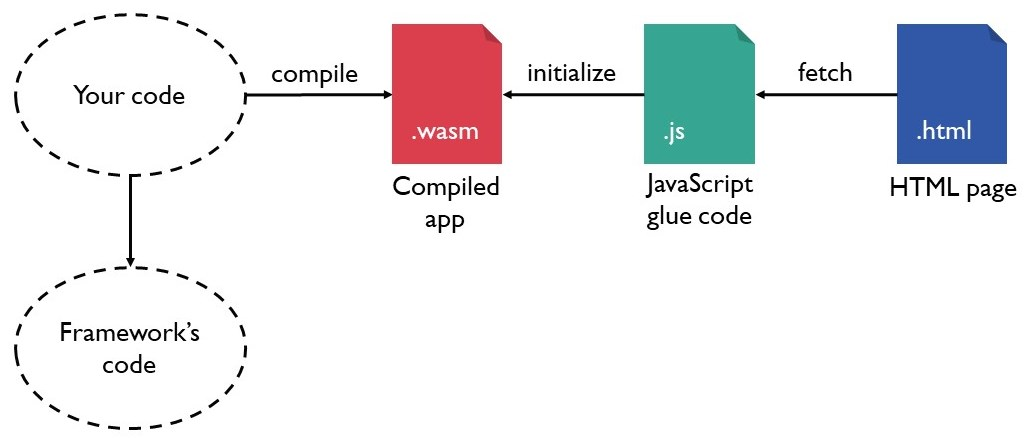
\includegraphics[width=13cm]{wasm}
				\caption{Proces využití WebAssembly pro webové aplikace \cite{wasm_fig}}
				\label{fig:wasm}
			\end{figure}
		\end{center}
		
		Postup pro získání bajtkódu i~lepícího kódu (který bude komunikovat mezi JS a~bajtkódem) lze postupovat následovně.
		
		Nejprve je potřeba přidat následující dependencies do \texttt{Cargo.toml}
		\begin{minted}{toml}
[target.'cfg(target_arch = "wasm32")'.dependencies]
tracing = "0.1.29"
tracing-subscriber = "0.2.25"
tracing-wasm = "0.2.0"
		\end{minted}
		
		Užitý syntax má význam v~přidávání crates specifických pro cílovou architekturu \texttt{wasm32}. Crate \texttt{tracing} není povinná, ale nastane-li chyba ze strany wasm bajtkódu, je schopna tuto chybu vypsat do vývojářské konzole webového rozhraní. Následně je nutno poskytnou speciální funkci, která bude vstupním bodem pro wasm
		\begin{minted}{rust}
#[cfg(target_arch = "wasm32")]
#[wasm_bindgen]
pub fn main_web(canvas_id: &str) {
	tracing_wasm::set_as_global_default();

	// *kód pro spuštění na webu*
}
		\end{minted}
		
		Nyní jen zbývá přidat následující do \texttt{Cargo.toml}
\begin{minted}{toml}
[lib]
crate-type = [ "cdylib", "rlib"]
		\end{minted}
		
		A nyní už je hotovo po stránce editování původního kódu a~lze přejít ke kompilování.
		\begin{minted}{bash}
cargo build --release --lib \
			-p muj_program \
			--target wasm32-unknown-unknown \
		\end{minted}
		
		Následně jee potřeba vygenerovat glue code. K~tomu lze použít programu \texttt{wasm-bindgen}. Ten se dá nainstalovat přes
		\begin{minted}{bash}
cargo install -f wasm-bindgen-cli
cargo update -p wasm-bindgen
		\end{minted}
		
		Poté ho lze použít na~vygenerovaný WASM soubor
		\begin{minted}{bash}
wasm-bindgen target/wasm32-unknown-unknown/release/muj_program.wasm \
			--no-modules \
			--no-typescript \
		\end{minted}
		
		Toto v~adresáři WASM souboru vygeneruje soubor \texttt{muj\_program\_bg.js}. Nyní se vezme tento soubor společně s~\texttt{muj\_program.wasm} a~oba jsou přesunuty do nové složky. V~této samé složce je nutno vytvořit html soubor, např. \texttt{index.html}, s~následujícím obsahem
		\begin{minted}{html}
<!DOCTYPE html>
<html>
<head>
	<title>Game of Life</title>
</head>
<body>
	<canvas id="app"></canvas>

	<script src="muj_program_bg.js"></script>
	<script>
		wasm_bindgen("./muj_program.wasm")
			.then(on_wasm_loaded)
			.catch(console.error);

		function on_wasm_loaded() {
			wasm_bindgen.main_web("app");
		}
	</script>
</body>
</html>
		\end{minted}
		
		Díky minimálnímu kódu je načten bajtkód a~spuštěna dříve definované funkce \rust{main_web()} odkazující na~\texttt{canvas}, do kterého je GUI vykreslováno.
		
		Nyní však ještě není hotovo. Po otevření \texttt{index.html} ve webovém prohlížeči nebude aplikace fungovat. Při otevření konzole lze identifikovat vadu - CORS (Cross-origin resource sharing) chybu. Toto dává smysl - při pohledu na~soubor \texttt{index.html} lze zjistit, že funkce \rust{wasm_bindgen()} potřebuje načíst soubor \texttt{muj\_program\_bg.wasm} toto však nelze, nejsou-li soubory získány přes webový server. Jeden způsob by byl instalací webového serveru \texttt{basic-http-server}
		\begin{minted}{bash}
cargo install basic-http-server
		\end{minted}
		
		Ten lze využít (v adresáři s~webovými soubory) příkazem
		\begin{minted}{bash}
basic-http-server --addr 127.0.0.1:3000 .
		\end{minted}
		
		Nyní je celý proces hotov a~webovou aplikaci lze spustit na~adrese \linebreak\texttt{localhost:3000}.\cite{wasm_vid, wasm_gh}


\section{Tvorba programu - Hra života}
	\subsection{Vymezení cílů}
		Cílem této aplikace je naprogramovat cross-platform řešení pro uživatelem přizpůsobitelnou simulaci Hry života Johna Conwaye. Jedná se o "hru jednoho hráče", která je vizualizována jako dvojrozměrné pole buněk. Každá tato buňka je v~jakémkoliv čase právě v~jednom ze dvou stavů - mrtvá nebo živá. Čas v~simulaci je kvantifikován na~tzv. generace. To, zda mrtvá buňka v~další generaci oživne, nebo to, zda-li živá buňka zemře, podléhá nastaveným pravidlům hry, které se vážou na~počet živých sousedních buněk. Tradiční konfigurace se označuje jako S23/B3. To znamená, že aby živá buňka přežila, musí mít 2 nebo 3 živé sousedy a~aby mrtvá buňka oživla, musí mít právě 3 živé sousedy (nastane-li cokoliv jiného, poté buňka umře, respektive zůstává mrtvá).\cite{conway}.
		\begin{center}
			\begin{figure}[H]
				\centering
				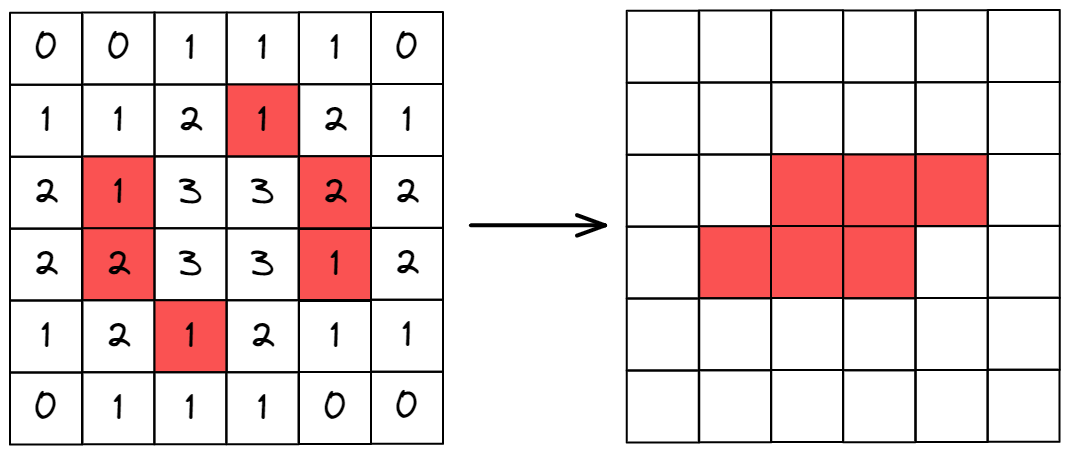
\includegraphics[width=.82\linewidth]{conway}
				\caption{Příklad vytvoření nové generace v~Conwayově Hře života, S23/B3}
				\label{fig:conway}
			\end{figure}
		\end{center}
	
		Aplikace by měla běžet na~všech signifikantních platformách a~měla by mít minimální systémové požadavky.
	
	\subsection{Výběr frameworku}
		Bohužel co se GUI frameworků týče, Rust ještě není dostatečně vybaven. Obecně není příliš velký výběr a~z toho mála, co je, jsou všechny immediate mode. Respektive existují ve vývoji i~retained mode, avšak ty jsou ve velice útlém a~experimentálním stádiu.

		Rozdíl mezi těmito dvěma je ten, že retained mode GUI si uchovává vzhled okna aplikace, a~tedy je toto okno přerenderováno pouze tehdy, nastane-li v~jeho vzhledu nějaká změna. Kdežto immediate mode GUI si neuchovává nic a~každý jeden snímek je znovu renderován. Na~základě těchto poznatků lze vyvodit, že pokud se vzhled okna má často měnit (jako třeba nějaká hra), poté je vhodnější immediate mode, kdežto u~desktopových aplikací, jejichž vzhled se moc nemění (jako třeba nějaké formuláře), je vhodnější retained mode. Tato aplikace má být něco mezi těmito dvěma paradigmaty - a~tedy limit daný omezeným výběrem není tak veliký takový problém.
		\begin{center}
			\begin{figure}[H]
				\centering
				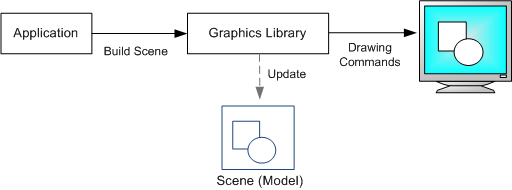
\includegraphics[width=.82\linewidth]{imm_mod}
				\caption{Diagram procesu renderování immediate mode\cite{imm_mod}}
				\label{fig:imm_mod}
			\end{figure}
		\end{center}
		\begin{center}
			\begin{figure}[H]
				\centering
				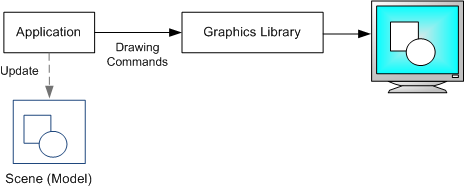
\includegraphics[width=.82\linewidth]{ret_mod}
				\caption{Diagram procesu renderování retained mode\cite{ret_mod}}
				\label{fig:ret_mod}
			\end{figure}
		\end{center}
		
		Frameworkem, který jsem nakonec zvolil je egui, a~to zejména kvůli tomu, že disponuje všemi funkcionality, které potřebuji - vykreslováním všech widgetů, které chci a~má excelentní podporu pro WebAssembly.\cite{egui}
	
	\subsection{Struktura / rozvržení}
		Po vytvoření projektu pomocí \texttt{cargo new gol} je vytvořeno následně několik dalších složek a~souborů tak, že struktura souborů bude vypadat následovně:
		\begin{center}
		\begin{forest}
			for tree={
			font=\ttfamily,
			grow'=0,
			child anchor=west,
			parent anchor=south,
			anchor=west,
			calign=first,
			edge path={
				\noexpand\path [draw, \forestoption{edge}]
				(!u.south west) +(7.5pt,0) |- node[fill,inner sep=1.25pt] {} (.child anchor)\forestoption{edge label};
			},
			before typesetting nodes={
				if n=1
				{insert before={[,phantom]}}
				{}
			},
			fit=band,
			before computing xy={l=15pt},
			}
		[gol
			[.git
			[\vdots]
			]
			[code
			[resources
				[logo.png]
			]
			[src
				[main.rs]
				[lib.rs]
			]
			[target
				[\vdots]
			]
			[Cargo.toml]
			]
			[dest
			[]
			]
			[.gitignore]
			[build.py]
		]
		\end{forest}
		\end{center}

		\begin{itemize}
			\item \texttt{code} slouží pro zdrojový kód a~související zdroje
			\begin{itemize}
				\item \texttt{resources} slouží pro obrázky, které program využívá
			\end{itemize}
			\item \texttt{dest} slouží pro exportované aplikace
			\item \texttt{build.py} je skript pro export aplikací
		\end{itemize}
		
	\subsection{Logická struktura}
		Jak je u~větších projektů zvykem, samotný soubor \texttt{main.rs} je jakousi pouhou „vstupní branou“, která pouze inicializuje program. 
		
		\begin{minted}{rust}
use eframe::{run_native, NativeOptions};

// Game struct v~lib.rs
use gol::Game;

fn main() {
	// vytvoření instance hry
	let mut game = Game::new(20);

	// spuštění GUI prostřednictvím herních structu
	let win_option = NativeOptions::default();
	run_native(Box::new(game), win_option);
}
		\end{minted}
		
		Čiže se jen odkáže na~položky v~jiných modulech, v~tomto případě v~\texttt{lib.rs}. V~něm bude struktura následující
		\begin{minted}{rust}
// import komunitních beden
use eframe::{ /* ... */ };

// objekt buňky
#[derive(Default)]
struct Cell {
	pub is_alive: bool,
}

// herní objekt
pub struct Game {
	/* ... */
}

impl Game {
	// --------------------------------------
	//      Tvorba
	// --------------------------------------

	// pomocná funkce pro generování reprezentace pole s~buňkami
	fn generate_board(size: usize) -> Vec<Vec<Cell>> { /* ... */ }

	// vytvoření instance hry
	pub fn new(size: usize) -> Game { /* ... */ }

	// --------------------------------------
	//      Manipulace
	// --------------------------------------

	// umožní změnit velikost hrací desky do spec. velikosti
	pub fn resize_to(&mut self, size: usize) { /* ... */ }

	// nastaví náhodný stav buněk
	pub fn randomize_cells(&mut self, factor: u8) { /* ... */ }

	// změní stav specifikované buňky
	pub fn change_cell_state(&mut self, cell: (usize, usize)) { /* ... */ }

	// vrátí pozici (ne)kliknuté buňky
	fn get_clicked_cell(&self, pos: Pos2, rect: Rect) -> Option<(usize, usize)> { /* ... */ }

	// --------------------------------------
	//      Herní logika
	// --------------------------------------

	// získá počet živých sousedů buňky
	fn get_neighbor_count(&self, pos: (i32, i32)) -> u8 { /* ... */ }

	// vytvoří novou desku na základě pravidel
	pub fn iterate(&mut self) { /* ... */ }

	// --------------------------------------
	//      Kontroléry, komunikace s GUI
	// --------------------------------------

	// rozhodování o možnosti další iterace v závislosti na konf.
	pub fn handle_iterate(&mut self, ui: &mut Ui) { /* ... */ }

	// přidělí místo pro pole s buňkami
	fn allocate_space_for_cells(&self, ui: &mut Ui) -> (Id, Rect) { /* ... */ }

	// vykresluje pole s buňkami
	fn show_cells(&mut self, ui: &mut Ui, rect: Rect) { /* ... */ }
}

// egui vyžadouje implementaci `App` pro daný herní objekt
impl App for Game {
	// vykreslování
	fn update(&mut self,
				ctx: &eframe::egui::CtxRef,
				_frame: &mut eframe::epi::Frame<'_>){
		egui::CentralPanel::default().show(ctx, |ui| { /* ... */ });
	}

	// název okna
	fn name(&self) -> &str { "Hra života" }
}
		\end{minted}
		
		Pro herní struct je tedy implementována požadovaná trait \rust{App}, které vyžaduje dvě metody. Zbylé implementované metody souvisejí s~logikou hry a~její funkčností. Zde však není vše, je také zapotřebí pár úprav pro WebAssembly. Konkrétně je nejprve nutno nahradit 2 funkcionality - sledování času a~generování náhodných čísel. Pro tyto dva úkony jsou ve výchozím stavu užívány crates \rust{std::time} a~externí crate \rust{rand} v~tomto pořadí. Ty je nutno nahradit WebAssembly podporujícími alternativami.
		\begin{minted}{rust}
#[cfg(not(target_arch = "wasm32"))]
use std::time::{SystemTime, UNIX_EPOCH};

#[cfg(target_arch = "wasm32")]
use wasm_timer::{SystemTime, UNIX_EPOCH};
		\end{minted}
		
		Ještě je nutno označit v~\texttt{Cargo.toml} \texttt{lib} pro podpur WASM
		\begin{minted}{rust}
[lib]
crate-type = [ "cdylib", "rlib"]
		\end{minted}
		
		Tato část by byla hotova a~již stačí vytvořit vstupní bod pro WebAssembly (tj. funkci, na~kterou se JavaScript gluecode napojí)
		\begin{minted}{rust}
#[cfg(target_arch = "wasm32")]
use eframe::wasm_bindgen::{self, prelude::*};

#[cfg(target_arch = "wasm32")]
#[wasm_bindgen]
pub fn main_web(canvas_id: &str) {
	let mut game = Game::new(20);
	game.randomize_cells(40);

	tracing_wasm::set_as_global_default();
	eframe::start_web(canvas_id, Box::new(game));
}
		\end{minted}
		
		Již zbývá poslední krok - nastavit ikonu pro Windows pomocí \rust{winres} v~souboru \texttt{build.rs}
		\begin{minted}{rust}
#[cfg(windows)]
use winres::WindowsResource;

fn main() -> std::io::Result<()> {
	#[cfg(windows)] {
	WindowsResource::new()
		.set_icon("resources/logo.ico")
		.compile()?;
	}

	Ok(())
}
		\end{minted}
		
		A nastavit, aby se na~Windows neotevíralo okno příkazového řádku, tedy přidat do hlavičky \rust{main.rs}
		\begin{minted}{rust}
#![windows_subsystem = "windows"]
		\end{minted}


\section{Závěr}
	Se znalostí informací zde obsažených lze již přejít ke konstrukci i~ lehce komplikovanějších projektů. Avšak to samozřejmě požaduje čtení dokumentace a~vyhledávání. Proto bych chtěl ještě zmínit zdroje, které mohou tomuto dopomoci.
	\begin{itemize}
		\item Rust cookbook\cite{cookbook} - soubor mnoha příkladů pro specifické úkony jako čtení že souborů, parsování CLI argumentů, interakce s~databázemi, ad.
	\end{itemize}
	
	V~příloze č. 2 přikládám navíc seznam několika frameworků a~crates, které lze využít pro různé úkony.


%\printbibliography[title={Seznam použité literatury},heading={bibintoc}]
\bibliographystyle{unsrt}
\bibliography{literatura}

\section{Přílohy}
	\subsection{Konvence názvů}
		\hypertarget{konvence_nazvu}{}


		\subsubsection*{\texttt{snake\_case}}
			\begin{itemize}
				\item souborů a~složek
				\item všechny typy kromě typů \texttt{struct}, \texttt{enum} a~\texttt{trait}
				\item makra
				\item metody a~funkce
			\end{itemize}


		\subsubsection*{\texttt{CamelCase}}
			\begin{itemize}
				\item typy \texttt{struct}, \texttt{enum} a~\texttt{trait}
			\end{itemize}


		\subsubsection*{\texttt{UPPER\_CASE}}
			\begin{itemize}
				\item konstanty
				\item generické parametry
			\end{itemize}


		\subsubsection*{\texttt{lowercase}}
			\begin{itemize}
				\item lifetime
			\end{itemize}


		\subsubsection*{Další}
			\begin{itemize}
				\item funkce generující nějaký typ, struct, atd. se mají jmenovat \rust{new}, popřípadě \rust{new_s_nejakym_detailem}
				
				\hypertarget{_}{}
			\end{itemize}\cite{convention}


	\subsection{Vybrané frameworky a~crates}
		\subsubsection*{Vývoj webu}
			\begin{itemize} 
				\item Actix-web - velice rychlý všestranný framework
				\item Rocket
				\item Warp
			\end{itemize}


		\subsubsection*{Interakce s~databázemi}
			\begin{itemize} 
				\item Rusqlite - interakce s~SQLite
				\item Postgres - interakce s~PostgreSQL
				\item R2d2 - platforma pro pooling databází jako MongoDB, MySQL a~četné množství dalších
				\item Diesel - ORM a~query builder
			\end{itemize}


		\subsubsection*{GUI}
			Rust prozatím nemá žádné nativní retained-mode, proto jsou všechny zde uvedené immediate-mode
			\begin{itemize} 
				\item imgui-rs - bindy pro Dear ImGui
				\item iced-rs
				\item egui
				\item SixtyFPS
				\item Relm - založeno na~GTK+
			\end{itemize}


		\subsubsection*{Ostatní crates}
			\begin{itemize}
				\item rand - generování pseudonáhodných čísel
				\item lazy\_static - vyhodnocování statických hodnot při runtime
				\item Serde - serializace a~deserializace, populární s~serde\_json pro převádění JSON objektů
				\item clap - parsování CLI argumentů
				\item tokio - asynchronní programování
				\item reqwest - posílání a~přijímání HTTP zpráv
				\item tungstenite - implementace WebSocketů
			\end{itemize}
\end{document}
